%===================================== CHAP 6 =================================
\chapter{Experimental Setup}\label{chapter_experimental_setup}

In this chapter we present an experimental setup for the solution approach suggested in Chapter \ref{chapter_solution_approach}. In the chapter we describe the data used in the thesis. Moreover, we provide numerical values for the parameters introduced in Chapter \ref{chapter_model_formulation} and \ref{chapter_solution_approach}, as well as a justification for these. 

\newpar

The chapter begins with a presentation and discussion of the data in Section \ref{exp_setup_data}. Then, in Section \ref{Exp_setup_Player_Performance_Prediction}, we elaborate on how parameters and input associated with the three different prediction models are decided. Section \ref{exp_setup_gamechips} provides the decisions on which gameweeks to consider the use of gamechips. Finally, in Section \ref{exp_setup_Value_Variance} the numerical values related to the risk handling are presented.

\section{Data} \label{exp_setup_data}
We have used data provided by the official website of Fantasy Premier League. A detailed record of such data for both the 2016/2017- and the 2017/2018 season is kept by \url{www.fantasyoverlord.com}. As we only have data for two seasons, we are only capable of training the model on one season, and test on the other. This is a drawback, since it is reasonable to assume that if more data were available the model could be improved further and more robust statements could be made. Elo values for each Premier League team are obtained from \url{www.clubelo.com}. In addition, Sportradar has provided odds and probabilities for the fixtures of the 2017/2018 season. 

\subsection{Processing of Player's Data}

\subsubsection{Injuries and suspensions}
Once a player is listed as injured and thus unavailable for the upcoming gameweek, his expected points are automatically set to zero in all the gameweeks in the sub-horizon. As the injury list is updated for each gameweek, a player's injury status can change when entering a new sub-horizon. Injury data is collected from \url{www.fantasypremierleague.com }, ahead of each gameweek. 

\newpar

As for injuries, suspensions are also accounted for by rewarding suspended players 0 expected points in the gameweeks where they are suspended. A player may be suspended for up to three games when receiving a red card, depending on whether it was a direct red card or not. Further, players are subject to a match ban when receiving their 5th, 10th or 15th yellow card of the season. In addition, a player can be suspended by the English Football Association if he is found guilty of unsportsmanlike conduct. 


\subsubsection{Promoted teams}
Gathering data for newly promoted teams is difficult, as there does not exist Fantasy Premier League data for the English Championship. In addition, it requires a lot of computational work in order to compare performances in the English Championship to the Premier League. Due to these difficulties, some simplifications are made. For the modified average and regression based model, players on newly promoted teams are not considered in the first gameweek of the 2017/2018 season. If a player was transferred to a promoted team ahead of the season, and he played in the Premier League in the previous season, the player would then be included from the start of the season For the odds method data exists for newly promoted teams as well. It is worth noticing that in the modified average method, newly promoted teams are regarded from the beginning of the season in the sense that they are taken into consideration when computing the Elo ratings. 

\subsubsection{Players transferred ahead of 2017/2018 season}
A question that arise with the international transfer window, is how new players are going to perform in another league in a different country. We have decided to handle such players in the same way as with newly promoted players, by not considering them until they have featured in a gameweek. Other interesting approaches include forecasting based on their performance in the foreign league or comparing them to players of the same cost. However, comparison is a demanding task as it must be done for several leagues, including the Spanish La Liga, the Italian Serie A, the German Bundesliga, the Dutch Eredivisie etc. In general, the decision of not including players when data is missing is supported by the fact that we aim to test how the different approaches perform, and including such players introduce more uncertainty.


\subsubsection{Irregular gameweeks}
For blank gameweeks, expected points are set to 0 for players that are not featured. For double gameweeks, forecasts are made for both matches. We assume that information on whether a gameweek is blank or double is known 5 gameweeks in advance.

\newpage

\section{Player Performance Prediction}
\label{Exp_setup_Player_Performance_Prediction}

In this section, the three different prediction models are presented.

\subsection{Modified Average}
As mentioned in Section \ref{Player_Performance} the relative team strength factors are calculated according to the Elo values. The Elo values are updated for every gameweek, depending on the results in their previous games. An overview of the Elo values is attached in the appendix. 

\newpar

Table \ref{Field advantage} provides the calculated values for field advantages for the past six Premier League seasons. As observed, the field advantages are somewhat consistent with the home field advantage ranging from 1.105 to 1.149 and the away field advantage ranging from 0.851 to 0.895. Hence, simply taking the average over the past five seasons seems to yield an appropriate field advantage factor. 

\begin{table}[H]
\centering
\smaller
\begin{tabular}{|l|l|l|l|l|l|l|l|l|}
\hline
Season & 11-12    & 12-13   & 13-14    & 14-15    & 15-16 & 16-17 & 16-17 Avg & 17-18 Avg \\ 
\hline
Home advantage & 1.133 & 1.114 & 1.137 & 1.149 & 1.105 & 1.141 & \textbf{1.128} & \textbf{1.129}\\
\hline
Away advantage & 0.867 & 0.886 & 0.863 & 0.851 & 0.895 & 0.859 & \textbf{0.872} & \textbf{0.871}\\
\hline
\end{tabular}
\caption{Field advantages for previous 6 seasons.}
\label{Field advantage}
\end{table}

As for the point streak factor, the variables \textit{X} and \textit{Y} regarding whether a player is on a point streak, has to be decided. Since goalkeepers and defenders receive 4 points for keeping a clean sheet, all players get 3 points for an assist and midfielders and forwards get 5 and 4 points respectively for scoring a goal, the X variable should be set according to these numbers. Further, as a player gets 2 points for playing more than 60 minutes, it is appropriate to let the \textit{X} variable take a value of 5. Hence, if a player keeps a clean sheet, has an assist or scores a goal and in addition plays at least 60 minutes, he will receive enough points to be on a positive point streak given that he did not receive a yellow or red card. As for the \textit{Y} variable, a player that does not contribute with neither a goal, assist nor a clean sheet is awarded maximum 2 points. Thus, it is reasonable to set the \textit{Y} equal to 2 points. 


\subsubsection{Determining optimal forecasting horizon and optimization horizon}

With perfect information available, an optimization horizon 38 gameweeks (an entire season) is optimal. However, as perfect information is not available ahead of a gameweek, a sub-horizon of 38 gameweeks is not guaranteed to be optimal. In fact, considering all the uncertainty of future events, regarding goalscoring defenders, penalties saves, injuries etc. a sub-horizon of 38 gameweeks is unlikely to be optimal. In the following, we aim to determine an optimal sub-horizon based on the results from the 2016/2017 season. In addition, we decide how many gameweeks to look back when forecasting the future performances based on the previous averages.
\newpar
When determining the optimal optimization- and forecast horizon, we have decided that the forecast horizon should be at least as long as the optimization horizon. Moreover, the readers should be aware that the player predictions are expected to improve as the forecast horizon increases. For instance, consider the case when the forecast horizon is 6 gameweeks. As the data is tested on the 2016/2017 season, we only have data to consider the matches after gameweek 6 has been played. Hence, we get an opportunity of initially selecting the players that have performed best over the 6 first gameweeks. As an increase in forecast horizon allows one to select players that have initially performed well over more matches, one can argue that the player selection in 2016/2017 is biased to some degree. Due to this bias, we do not consider forecast horizons greater than 6 gameweeks. 
\newpar
Notice that only the testing data is biased. When we run the model for the 2017/2018 season, the previous gameweeks are simply set to previous gameweeks from the 2016/2017 season. Moreover, the reader should bear in mind that the parameters set are based solely on data from 2016/2017. Ideally, the parameters should have been tested over several seasons. 
\newpar
Figure \ref{fig:pen_4} displays the results when considering forecast horizons from 3 to 6 gameweeks as well as optimization horizons from 1 to 6 gameweeks.  Moreover, Table \ref{tab:pen_4_ill_trans} provides the numerical means displayed in Figure \ref{fig:pen_4} as well as average weekly illegal transfers made. 

\begin{figure}[H]
    \centering
    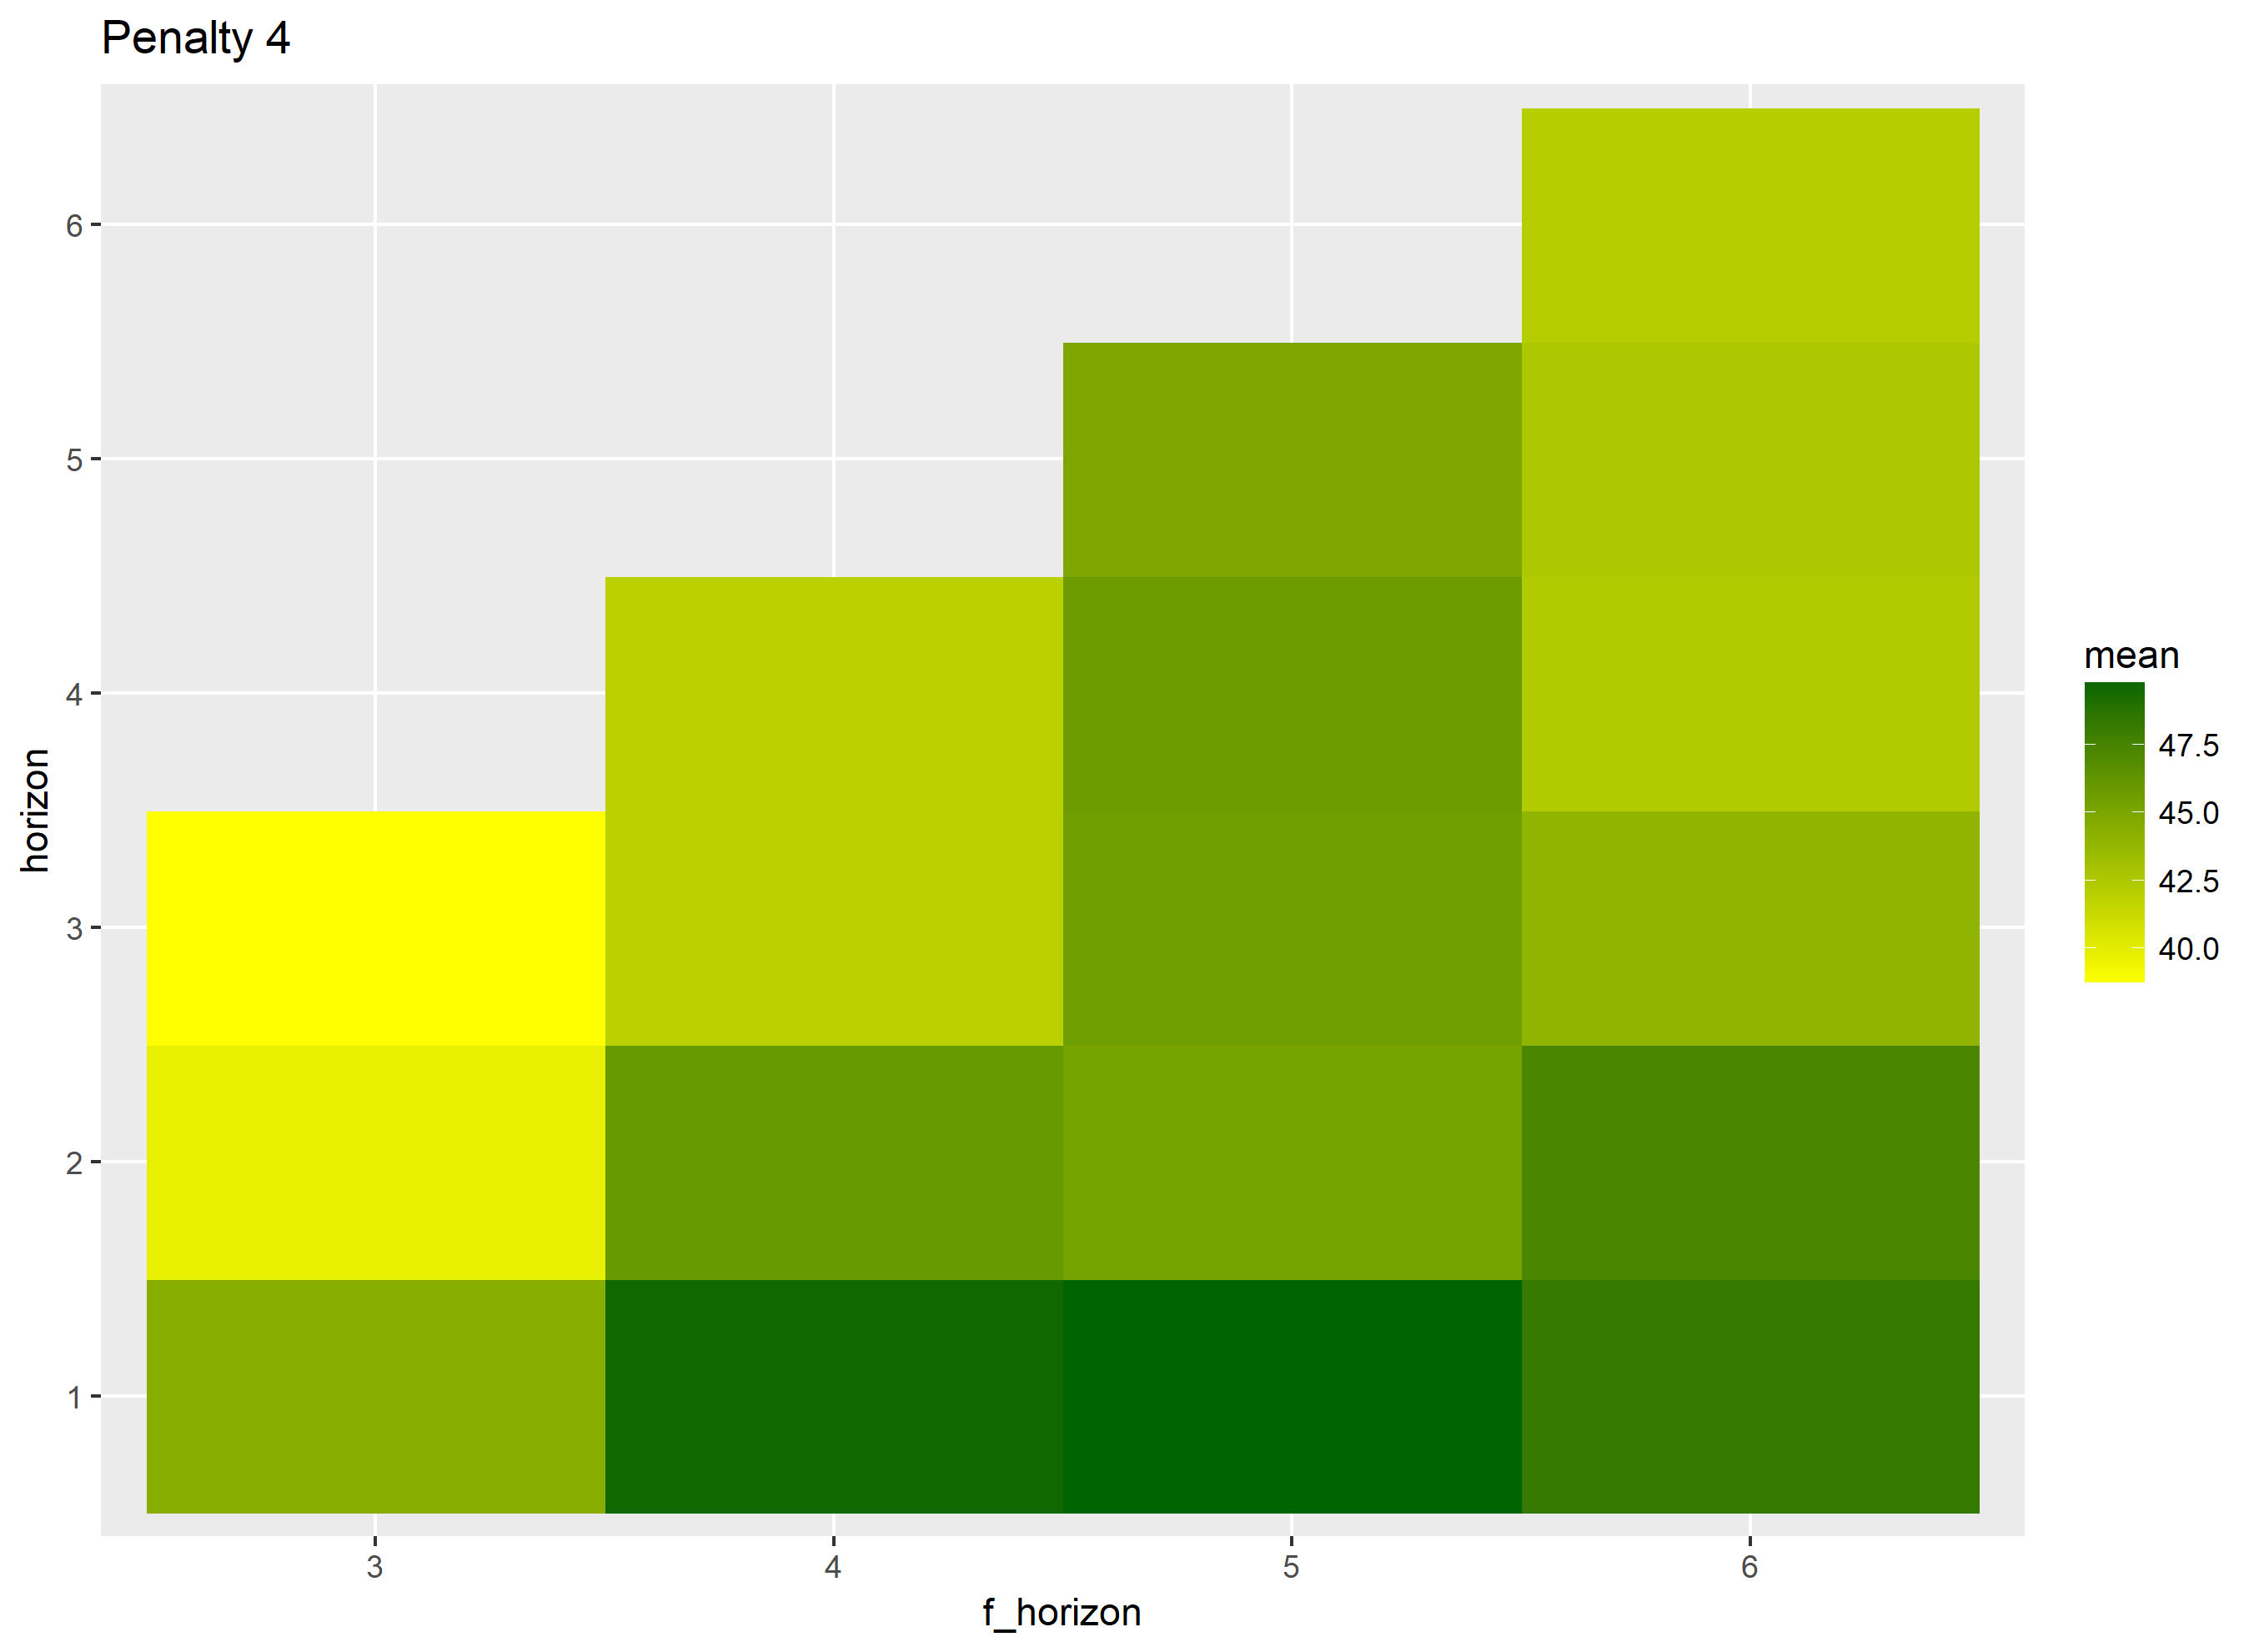
\includegraphics[scale=0.55]{fig/chapter_6/pen_4.png}
    \caption{Performance with changing optimization- and forecast horizons and constant transfer penalty 4}
\label{fig:pen_4}    
\end{figure}

\begin{comment}
\begin{table}[H]
\centering
\caption{Performance with changing optimization- and forecast horizons and constant transfer penalty 4}
\label{tab:pen_4}
\begin{tabular}{lllll}
penalty & horizon & f\_horizon & objective\_value & mean  \\
4       & 1       & 5          & 1644             & 49,82 \\
4       & 1       & 4          & 1684             & 49,53 \\
4       & 1       & 6          & 1544             & 48,25 \\
4       & 2       & 6          & 1513             & 47,28 \\
4       & 2       & 4          & 1562             & 45,94 \\
4       & 4       & 5          & 1509             & 45,73 \\
4       & 3       & 5          & 1504             & 45,58 \\
4       & 2       & 5          & 1491             & 45,18 \\
4       & 5       & 5          & 1481             & 44,88 \\
4       & 1       & 3          & 1555             & 44,43 \\
4       & 3       & 6          & 1407             & 43,97 \\
4       & 5       & 6          & 1361             & 42,53 \\
4       & 4       & 6          & 1355             & 42,34 \\
4       & 6       & 6          & 1350             & 42,19 \\
4       & 3       & 4          & 1428             & 42,00 \\
4       & 4       & 4          & 1428             & 42,00 \\
4       & 2       & 3          & 1394             & 39,83 \\
4       & 3       & 3          & 1357             & 38,77
\end{tabular}
\end{table}
\end{comment}



\begin{table}[H]
\centering
\caption{Illegal transfers with penalty 4}
\label{tab:pen_4_ill_trans}
\begin{tabular}{llllll}
penalty & horizon & f\_horizon & objective\_value & mean  & ill\_trans\_gameweek \\
4       & 1       & 5          & 1644             & 49.82 & 1.48       \\
4       & 1       & 4          & 1684             & 49.53 & 1.88       \\
4       & 1       & 6          & 1544             & 48.25 & 1.34       \\
4       & 2       & 6          & 1513             & 47.28 & 2.09       \\
4       & 2       & 4          & 1562             & 45.94 & 2.74       \\
4       & 4       & 5          & 1509             & 45.73 & 2.88       \\
4       & 3       & 5          & 1504             & 45.58 & 2.70       \\
4       & 2       & 5          & 1491             & 45.18 & 2.55       \\
4       & 5       & 5          & 1481             & 44.88 & 3.00       \\
4       & 1       & 3          & 1555             & 44.43 & 2.63       \\
4       & 3       & 6          & 1407             & 43.97 & 2.69       \\
4       & 5       & 6          & 1361             & 42.53 & 3.03       \\
4       & 4       & 6          & 1355             & 42.34 & 2.91       \\
4       & 6       & 6          & 1350             & 42.19 & 3.22       \\
4       & 3       & 4          & 1428             & 42.00 & 3.47       \\
4       & 4       & 4          & 1428             & 42.00 & 3.50       \\
4       & 2       & 3          & 1394             & 39.83 & 3.91       \\
4       & 3       & 3          & 1357             & 38.77 & 4.29      
\end{tabular}
\end{table}


As observed, the model reaches its best performances  with an optimization horizon of 1 gameweek combined with a forecast horizon between 4 and 6 gameweeks. 
However, obtaining a weekly mean of 49.82 points is considered rather poor. From Table \ref{tab:pen_4_ill_trans}, its observable that the model performs many penalized transfers.  In general, making more than 1 penalized transfer on average is considered a lot. As they deduct points from the total score, they have a huge impact on the overall rankings. Moreover, according to Table \ref{tab:pen_4_ill_trans}, the performances generally increases as the number of illegal transfers decreases. Hence, in the following we investigate how regulations on the penalty parameter affects the results.  

\subsubsection{Model run with different penalties}
In order to set the values of the parameters in a sensible way, a number of different combinations of the three parameters are tested on the 2016/2017 season. Figure \ref{Parameter_choice} provides an overview of how the mean value of points for the entire 2016/2017 season changes with different forecasting horizons, optimization horizons and penalty terms. Moreover, Table \ref{tab:top_10} provides the numerical values from the best 10 combinations in Figure \ref{Parameter_choice}.


\newpar

\begin{comment}
\textit{Avsnittet ovenfor må skrives mer utfyllende og inneholde mer diskusjon. Spesielt fra setningen "Frist, a sub-horizon of 3-4..." og utover. Viktige punker å få med: at dette er kun testet på en sesong og derfor må alt bli tatt med en klype salt. Man vil ikke teste for mer enn forecasting horizon på 6, siden da har man så få datapunker å basere seg på at det blir unfair å sammenlikne dens resultater med forecasting horizon på f.feks 2. Det skrives at sub-horizon på 3-4 ser ideell ut, men hvorfor? Det må skrives.}
\end{comment}


\begin{figure}[H]
    \centering
    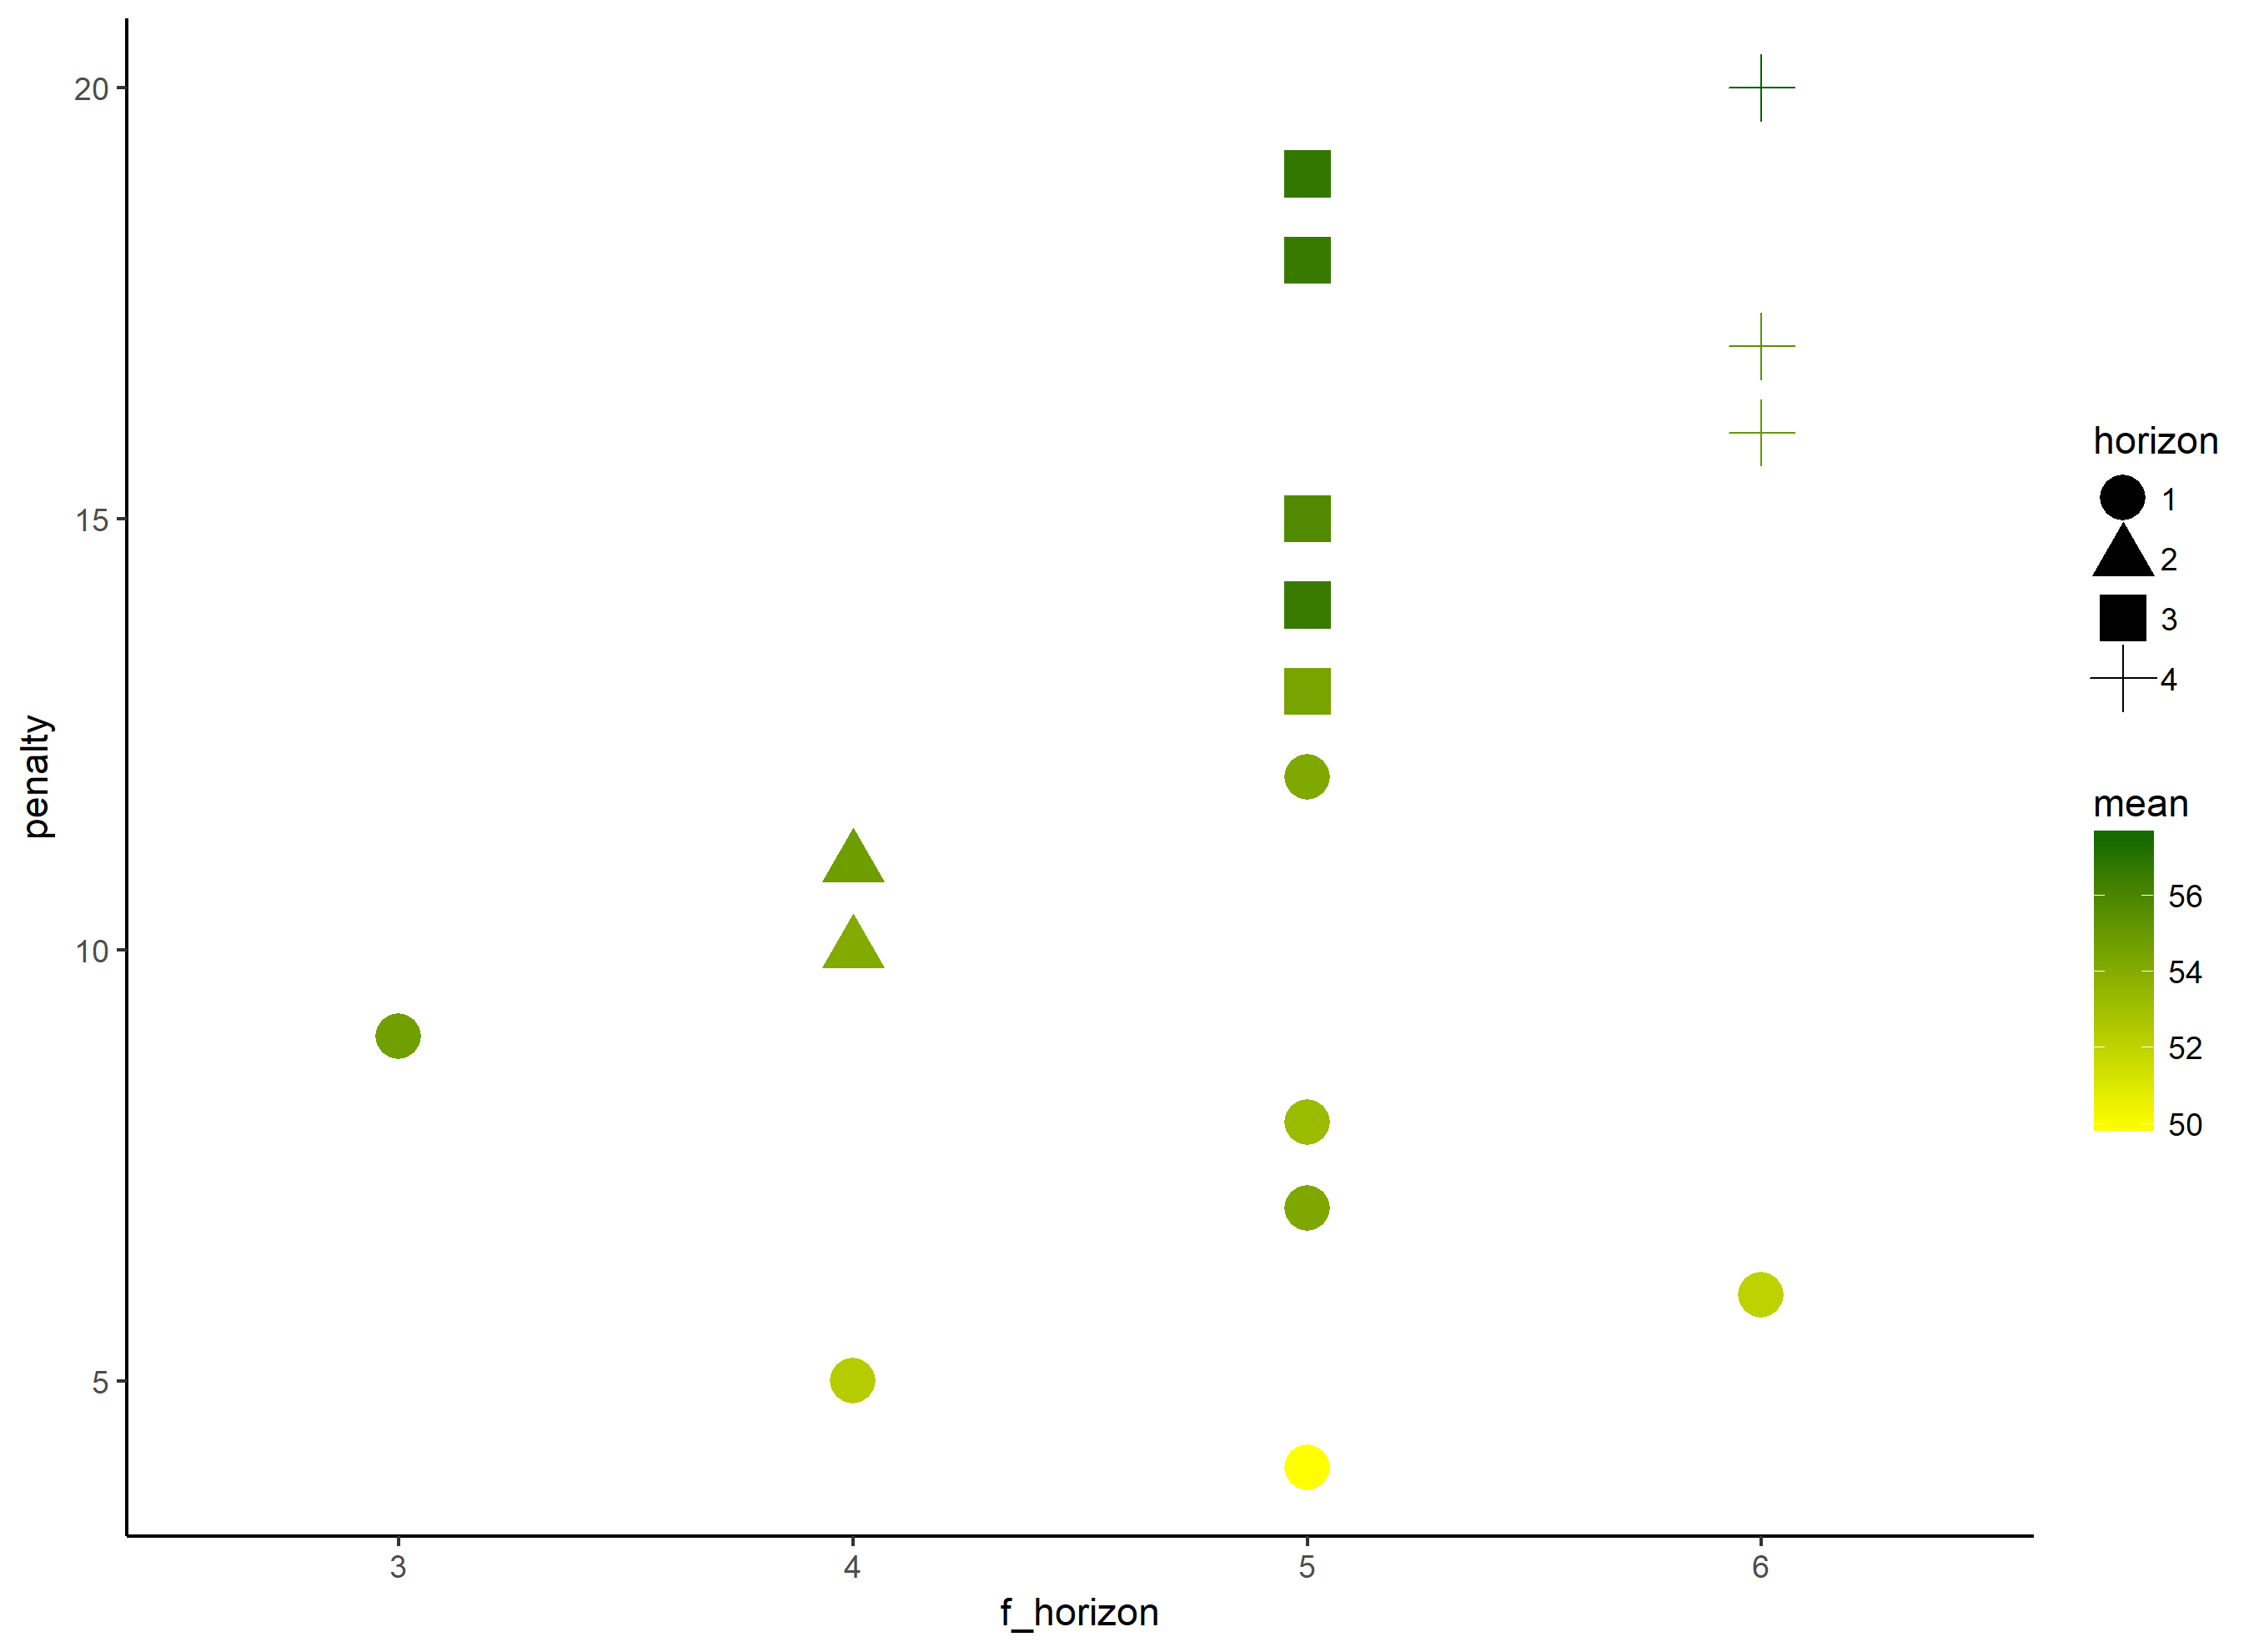
\includegraphics[scale=0.45]{fig/chapter_6/paramter_choice.png}
    \caption{Performance with different transfer penalties, optimization horizons and forecast horizons}
\label{Parameter_choice}    
\end{figure}

\begin{table}[H]
\centering
\caption{The 10 best combinations of parameters}
\label{tab:top_10}
\begin{tabular}{lllll}
Penalty & Horizon & Forecast Horizon & Total Points & Mean  \\
20      & 4       & 6                & 1851         & 57.84 \\
20      & 4       & 5                & 1899         & 57.55 \\
19      & 3       & 5                & 1875         & 56.82 \\
18      & 3       & 5                & 1869         & 56.64 \\
14      & 3       & 5                & 1868         & 56.61 \\
18      & 4       & 6                & 1808         & 56.50 \\
19      & 4       & 6                & 1806         & 56.44 \\
20      & 3       & 5                & 1860         & 56.36 \\
20      & 5       & 5                & 1851         & 56.09 \\
18      & 6       & 6                & 1793         & 56.03
\end{tabular}
\end{table}


In Figure \ref{Parameter_choice}, only the best run (maximum mean) for each different penalty value from 3 to 20 is plotted. According to the figure and Table \ref{tab:top_10}, optimization horizons of 3 to 4 gameweeks appear to be ideal, as they provide the combinations with the highest mean performances. Furthermore, penalties in the range of 14 to 20 yield the best results. As for the forecasting horizons, values of 5 and 6 gameweeks are clearly optimal. However, the latter is not unexpected due to the bias in player selection. 

\begin{figure}[H]
    \centering
    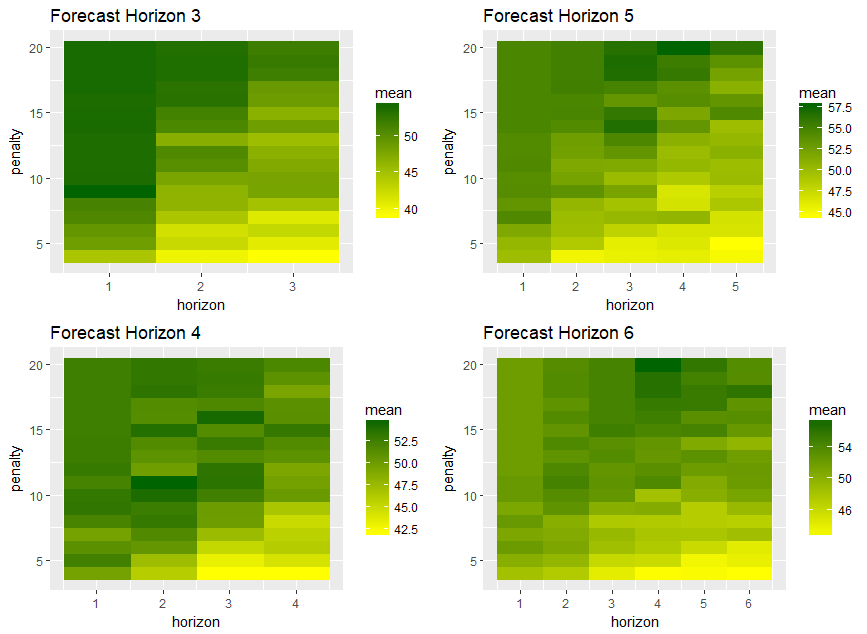
\includegraphics[scale=0.55]{fig/chapter_6/parameter_choice_fixed_f_hor.png}
    \caption{Performance with different transfer penalties and optimization horizons, but fixed forecast horizon}
\label{fig:fixed_f_hor}    
\end{figure}

\begin{table}[H]
\centering
\begin{tabular}{lllll}
Penalty & Horizon & Forecast Horizon & Total Points & Mean  \\
9       & 1       & 3                & 1914         & 54.69 \\
11      & 2       & 4                & 1863         & 54.79 \\
20      & 4       & 5                & 1899         & 57.55 \\
20      & 4       & 6                & 1851         & 57.84
\end{tabular}
\caption{The best combinations for each forecast horizon}
\label{tab:top_5}
\end{table}

\begin{comment}
In general, one can see that low transfer penalties combined with a high forecast horizon yield the poorest results. Furthermore, it seems like choosing 7 or 8 as the forecast horizon is the wiser choice. In addition, the transfer penalty should be set to a value above 10. Based on figure \ref{Parameter_choice}, a combination found in the center appears to be optimal, and the values $h = 6$, $f = 7$ and $p = 11$ are chosen. Also, a combination of $h = 4$, $f = 8$ and $p = 14$ yield good results. 
\newpar

\end{comment}

\begin{comment}

\subsubsection{Forecast Horizon 3}

\begin{figure}[H]
    \centering
    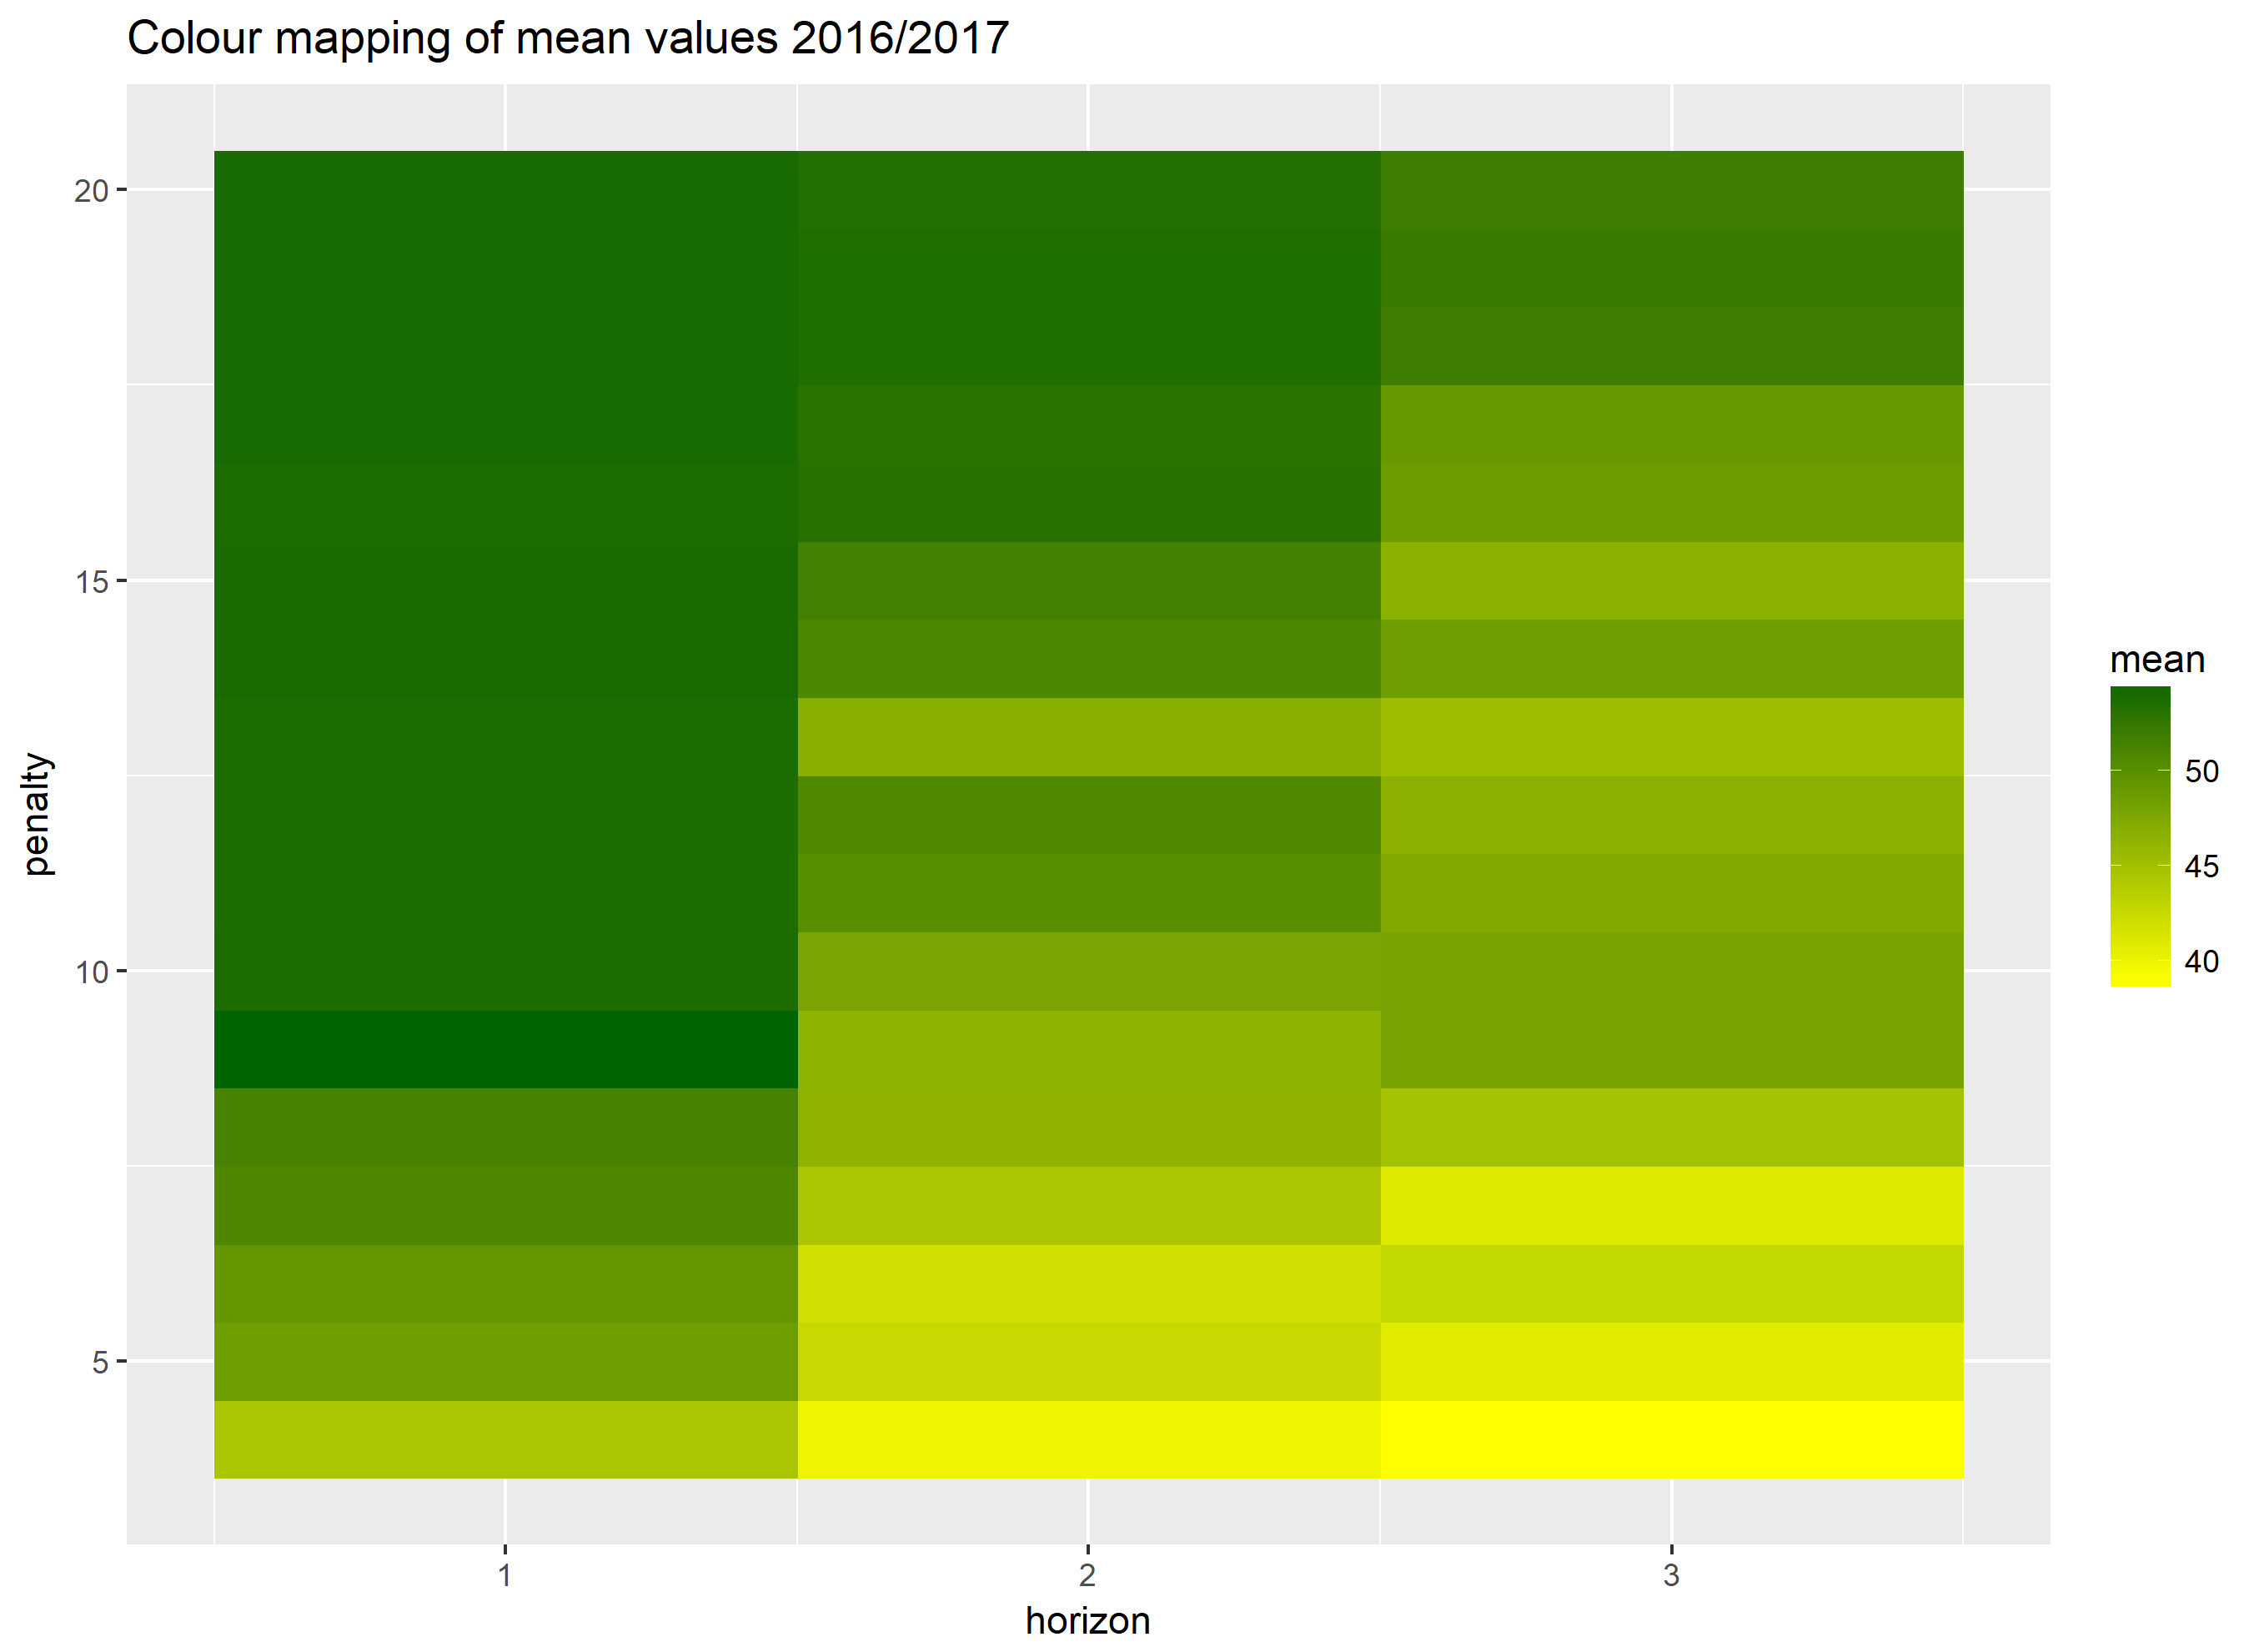
\includegraphics[scale=0.55]{fig/chapter_6/paramter_choice_3.png}
    \caption{Overview of total score with forecast horizon 3}
\label{fig:parameters_f_hor_3}    
\end{figure}

\subsubsection{Forecast Horizon 4}

\begin{figure}[H]
    \centering
    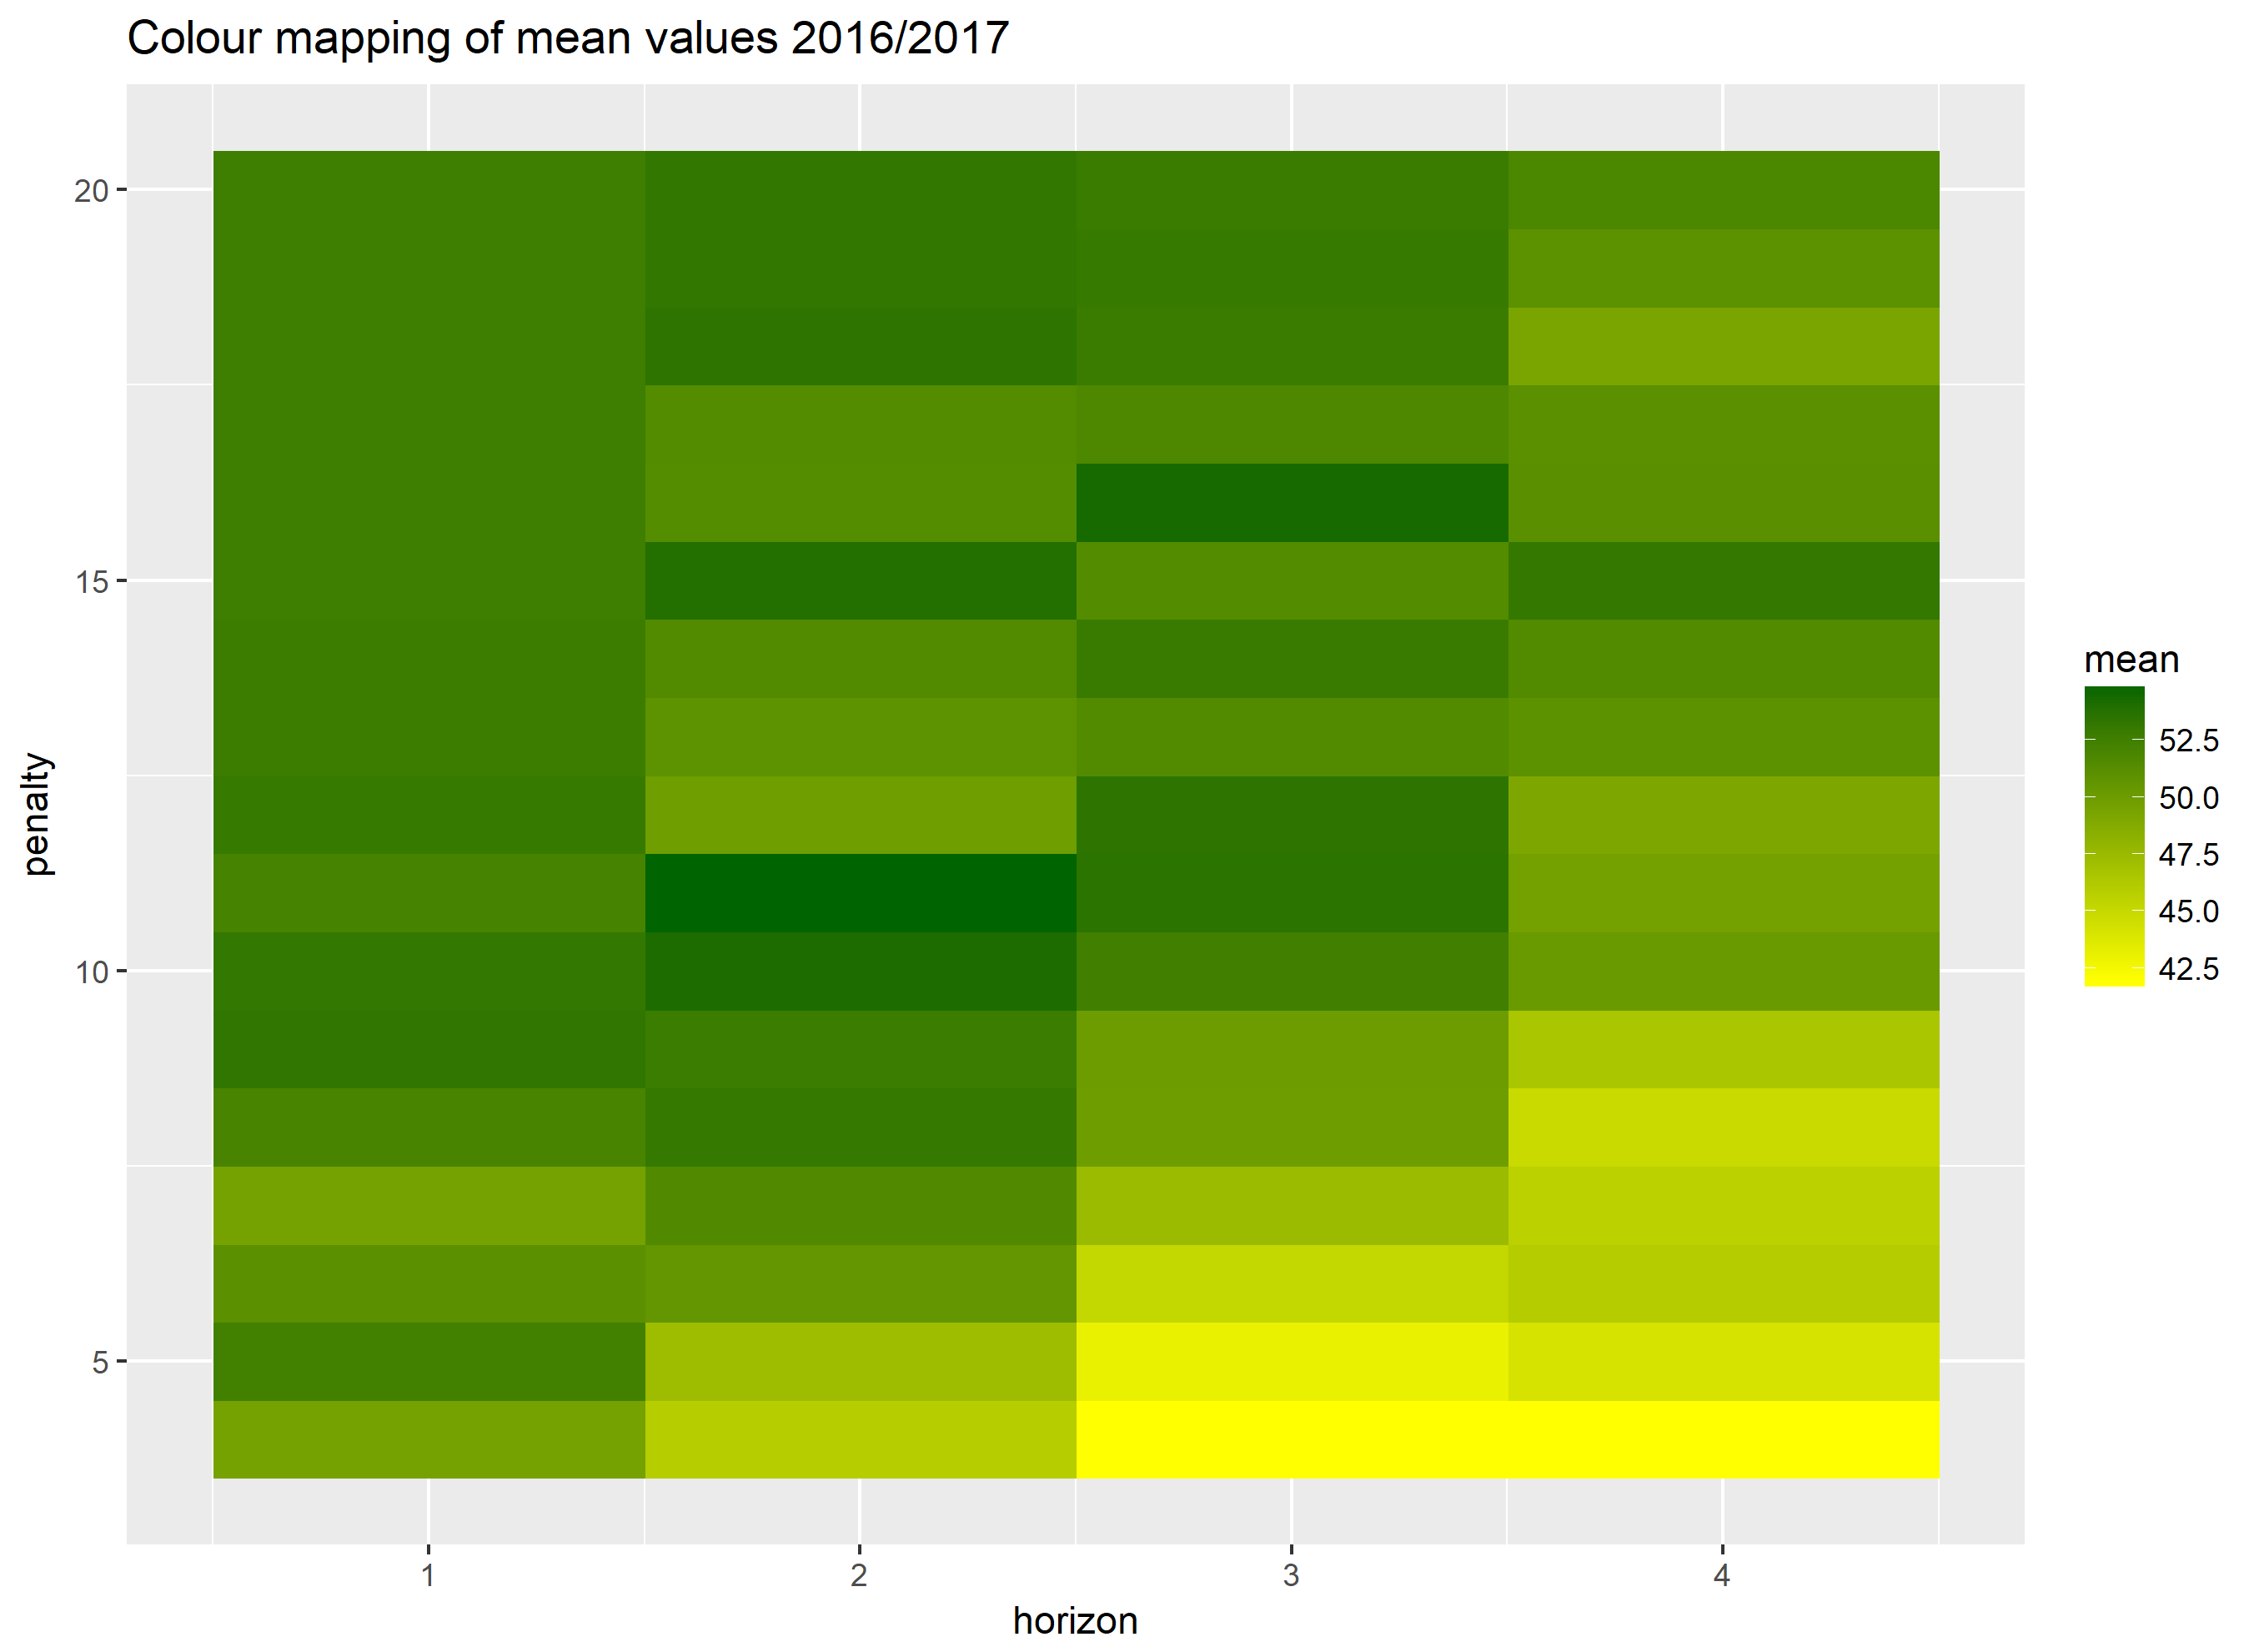
\includegraphics[scale=0.55]{fig/chapter_6/paramter_choice_4.png}
    \caption{Overview of total score with forecast horizon 4}
\label{fig:parameters_f_hor_4}    
\end{figure}

\subsubsection{Forecast Horizon 5}

\begin{figure}[H]
    \centering
    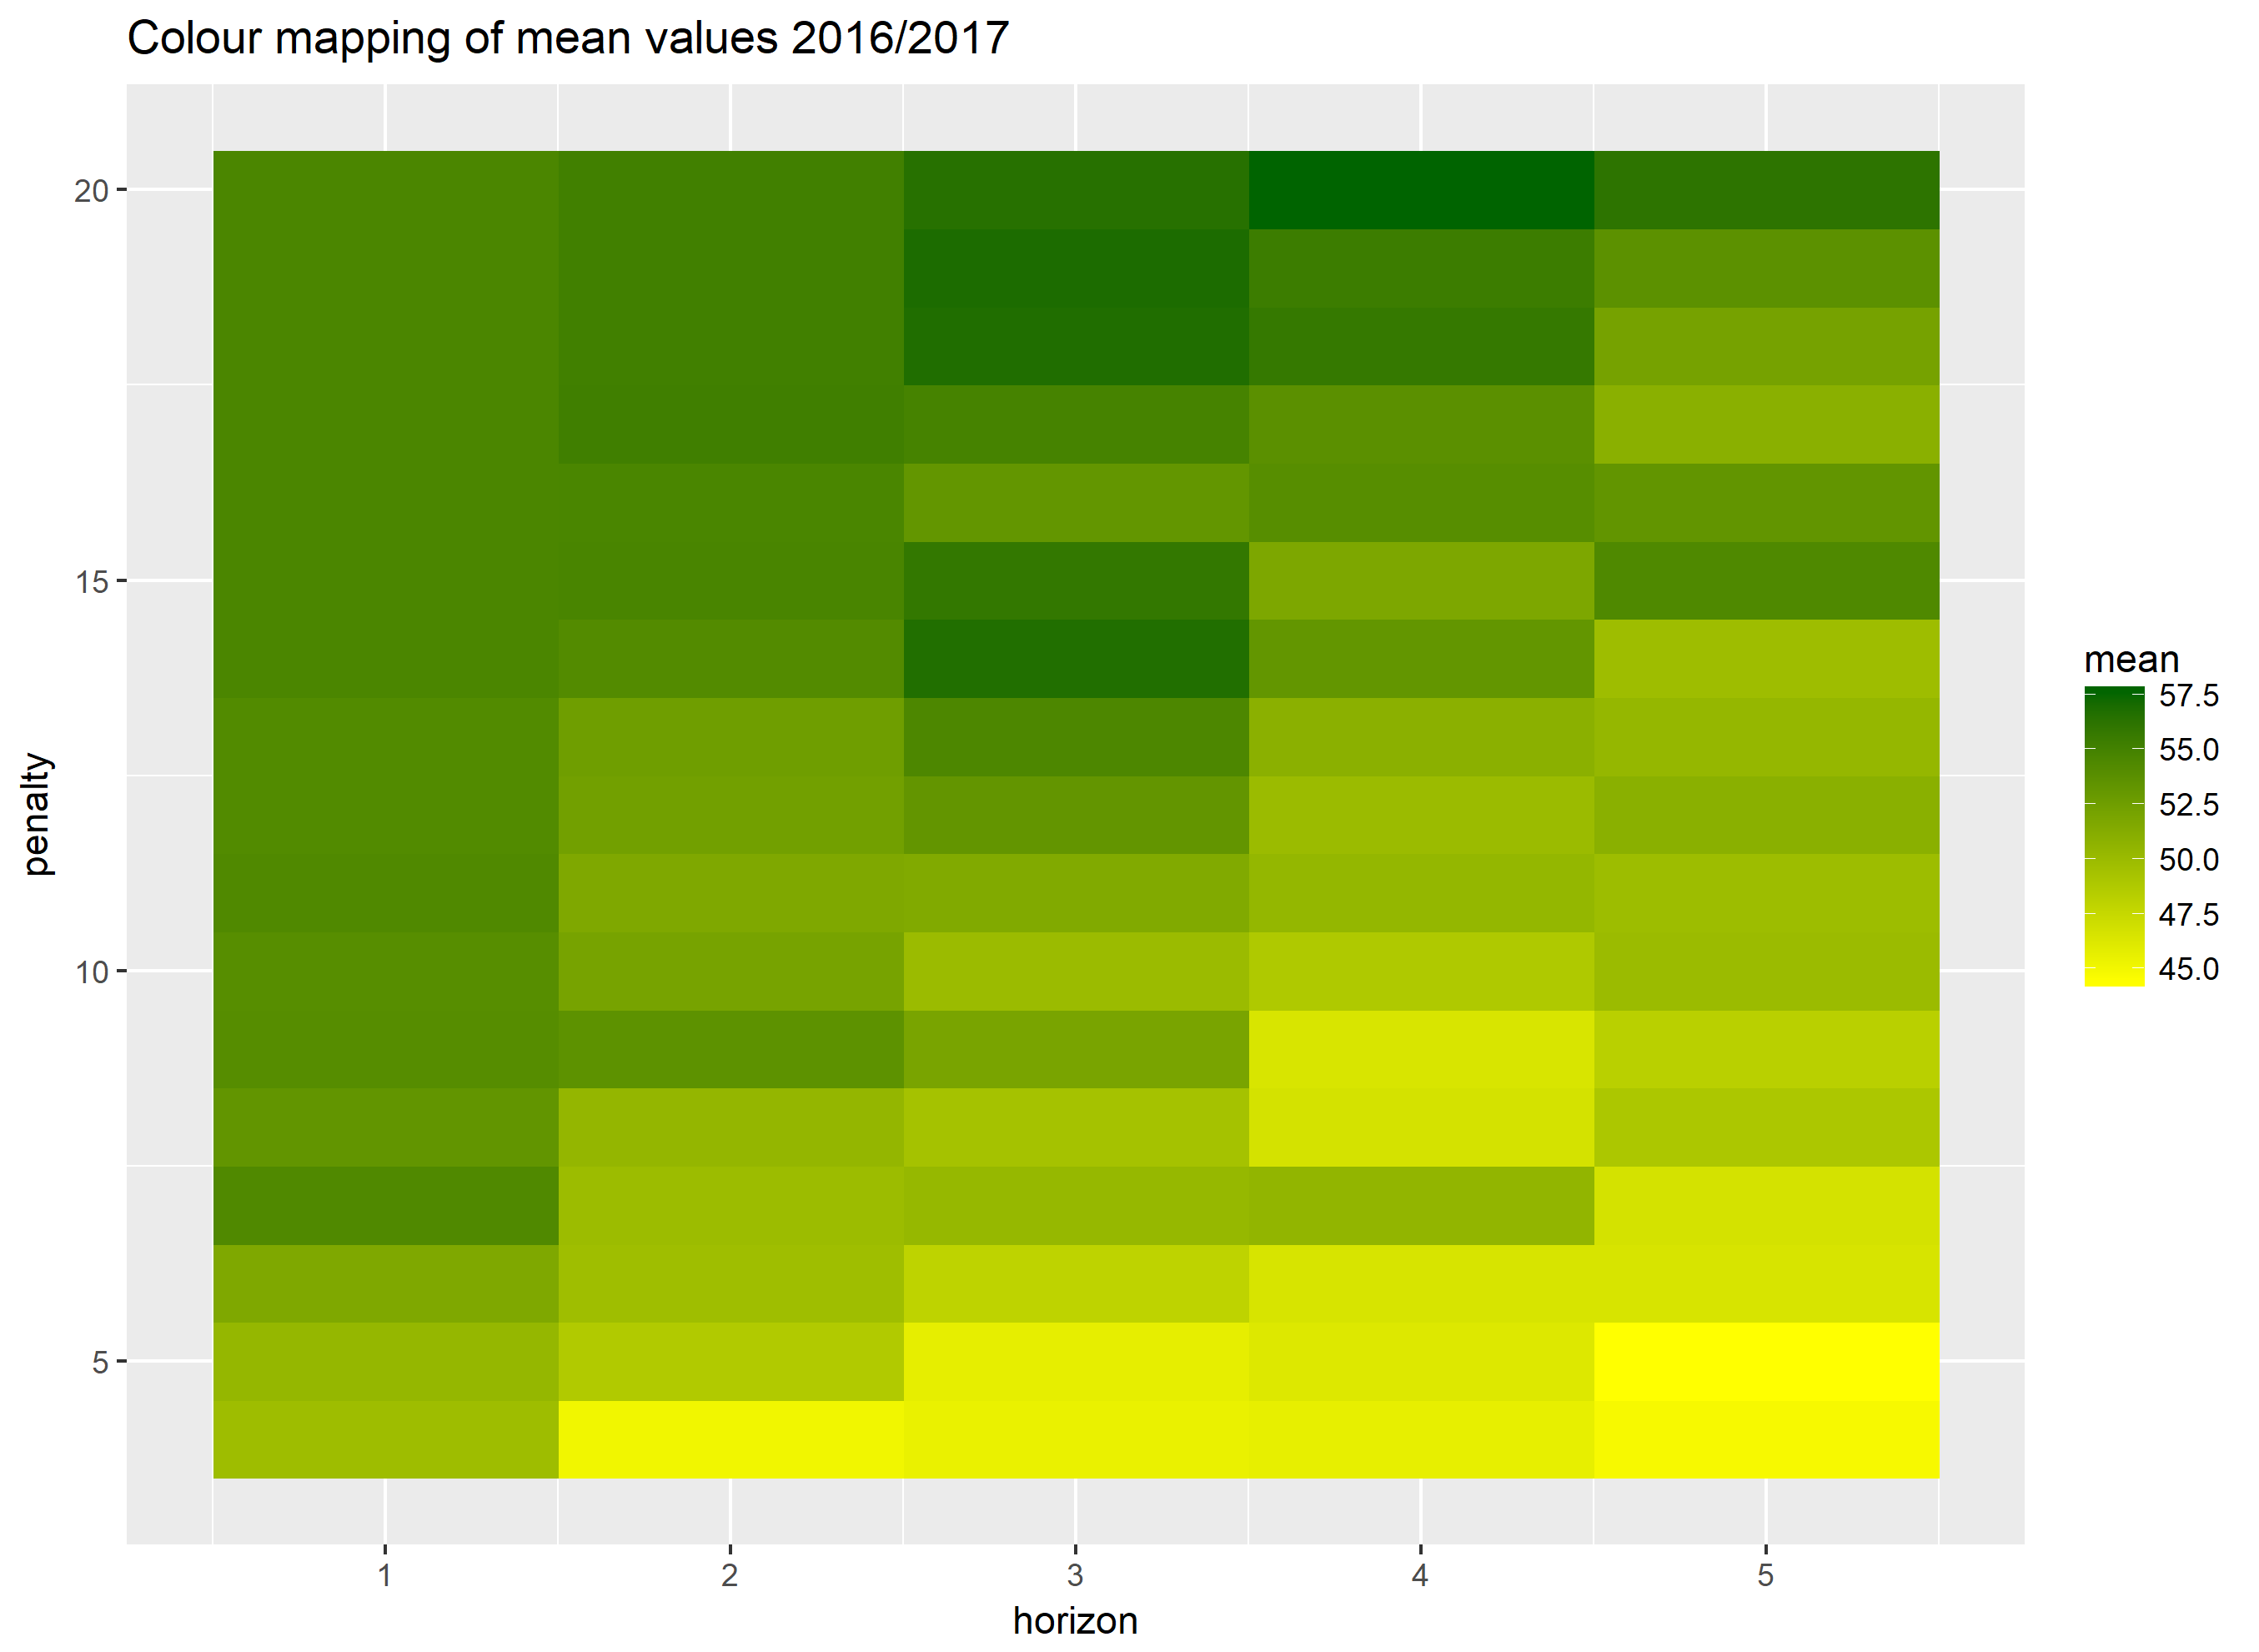
\includegraphics[scale=0.55]{fig/chapter_6/paramter_choice_5.png}
    \caption{Overview of total score with forecast horizon 5}
\label{fig:parameters_f_hor_5}    
\end{figure}

\subsubsection{Forecast Horizon 6}

\begin{figure}[H]
    \centering
    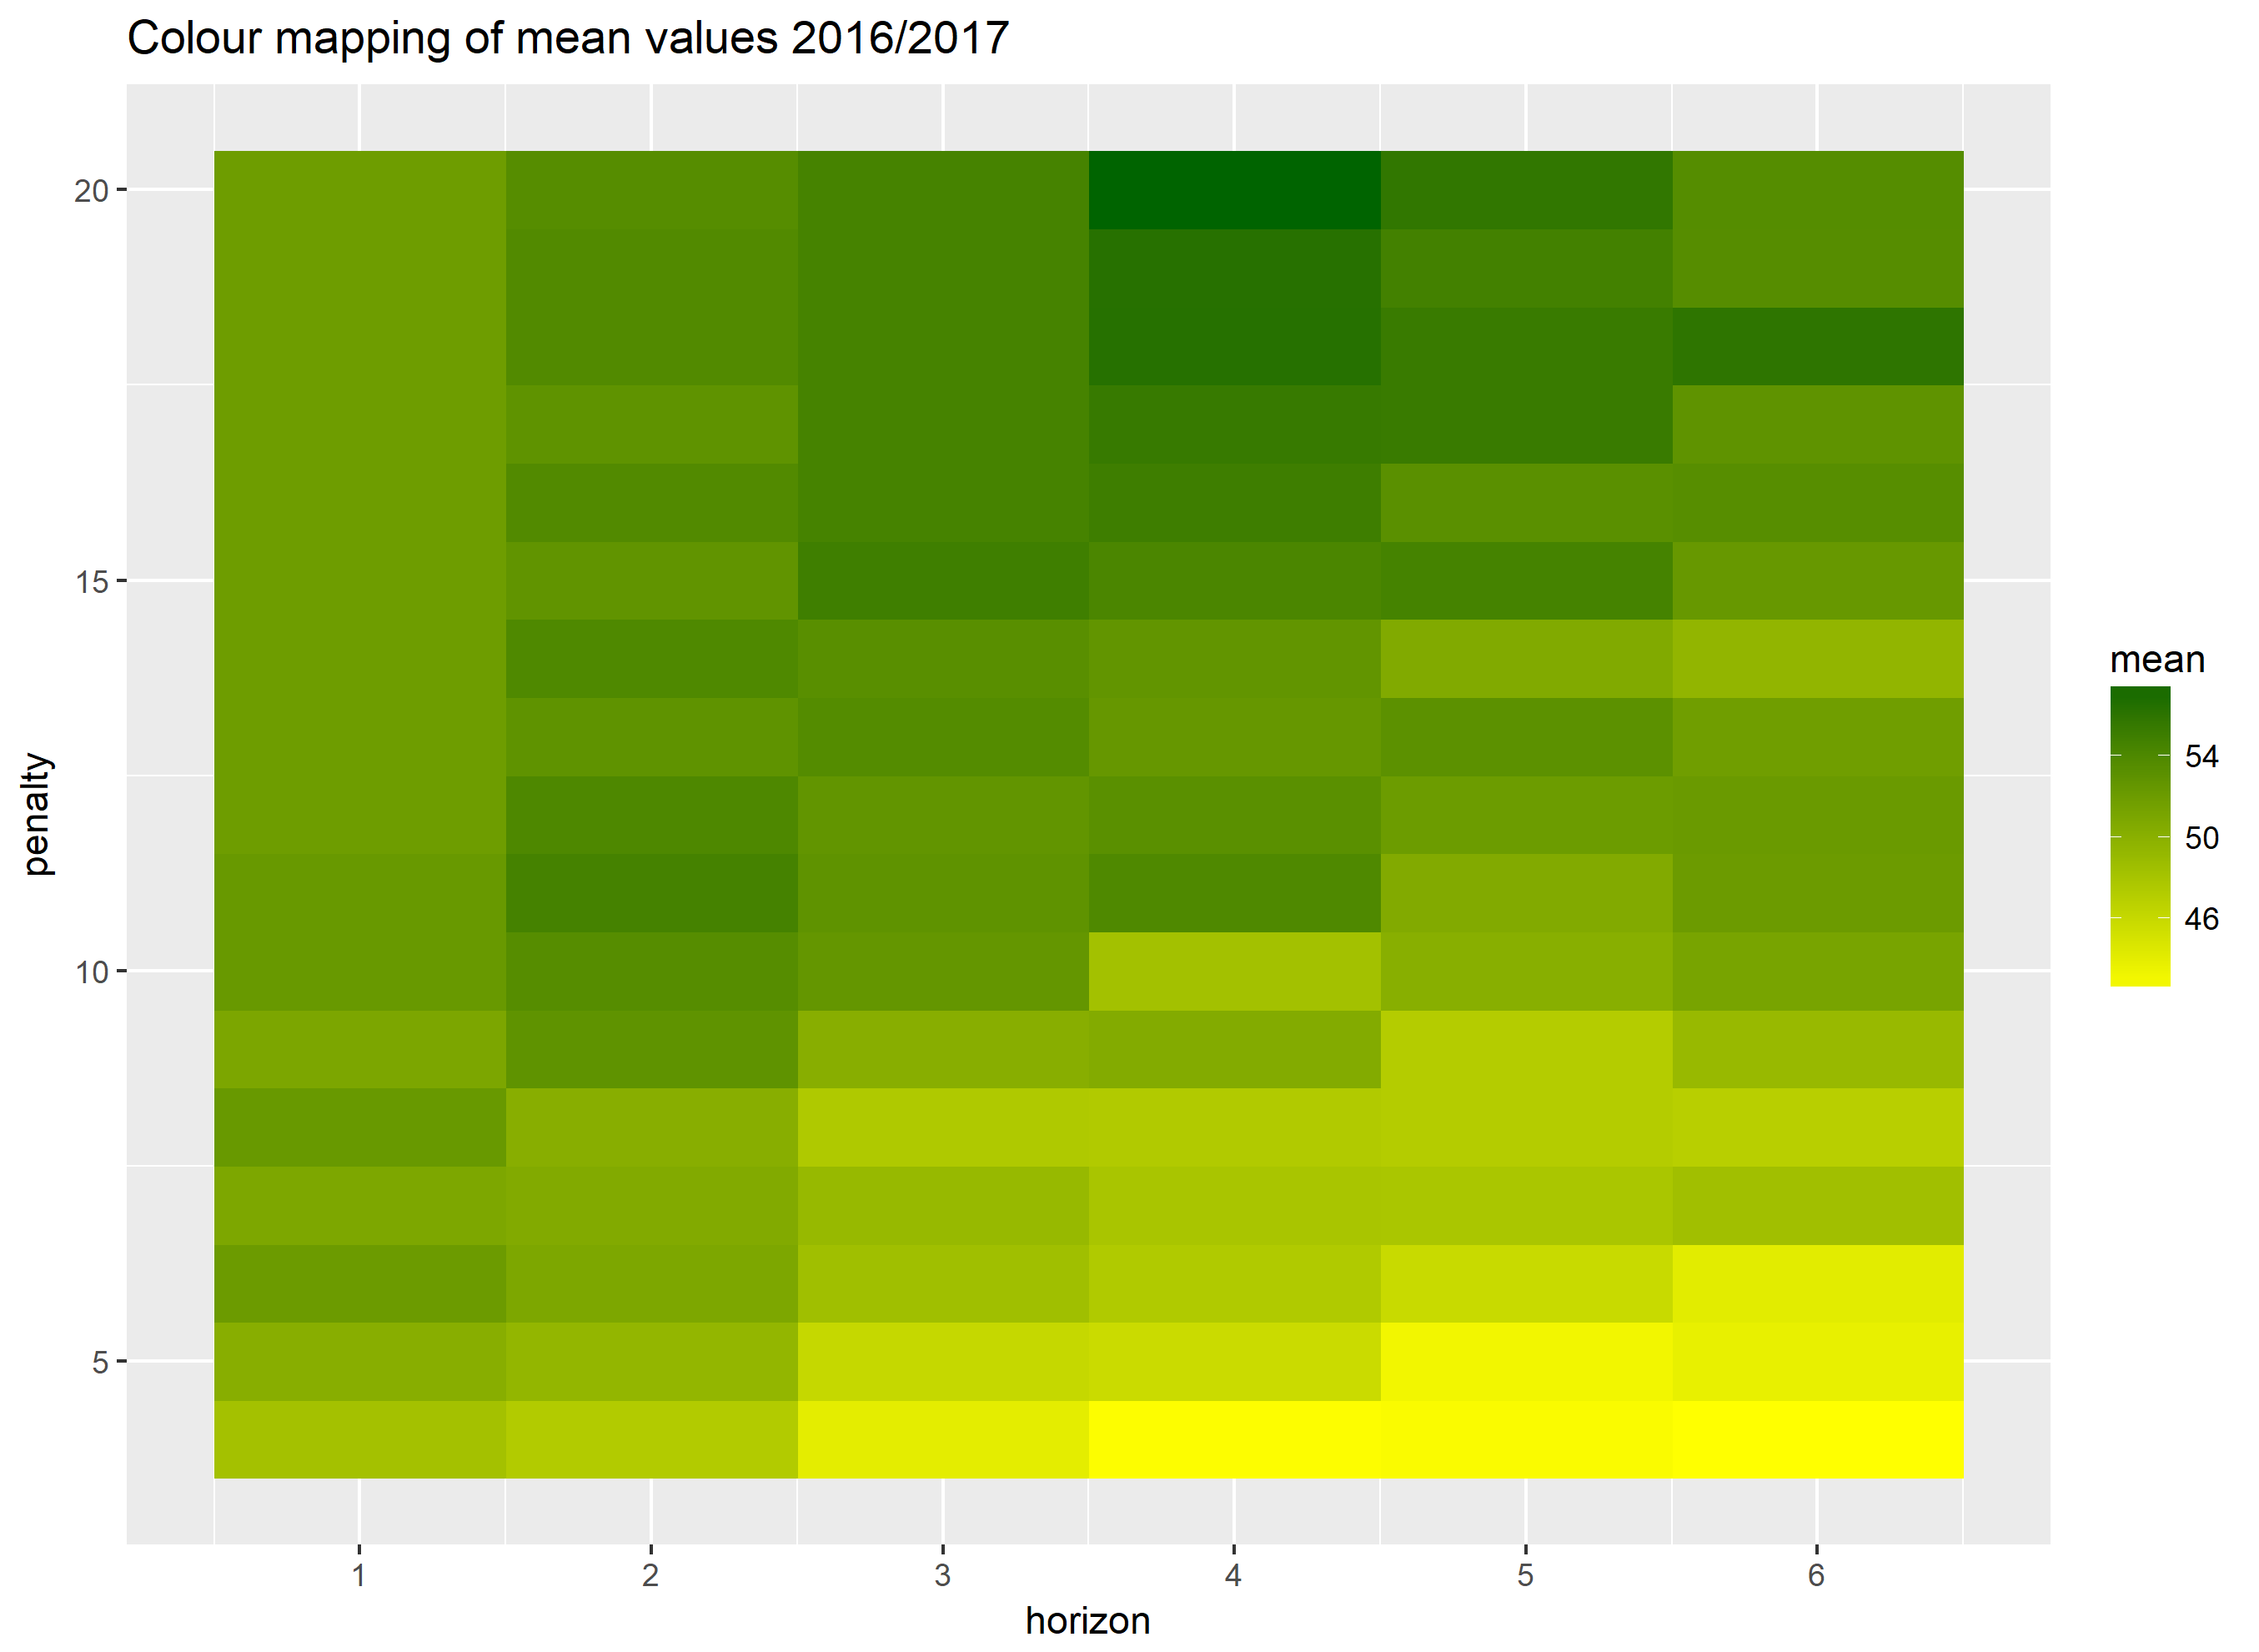
\includegraphics[scale=0.55]{fig/chapter_6/paramter_choice_6.png}
    \caption{Overview of total score with forecast horizon 6}
\label{fig:parameters_f_hor_6}    
\end{figure}

\end{comment}

Figure \ref{fig:fixed_f_hor} and Table \ref{tab:top_5} display the best combinations when the forecasting horizon is held fixed for 3 to 6 gameweeks. Clearly, forecast horizons of 5 and 6 gameweeks outperform those of 3 and 4 gameweeks. Moreover, Table \ref{tab:top_10} shows that a forecast horizon of 6 gameweeks combined with a optimization horizon of 4 gameweeks and a transfer penalty of 20 yields the highest mean for the 2016/2017 season. However, the next 4 top means are achieved with a forecast horizon of 5 gameweeks. Considering this, combined with the fact that an increasing forecast horizon yield biased player predictions, we find it appropriate to select 5 gameweeks as the optimal forecast horizon for the 2017/2018 season. Additionally, according to Figure \ref{fig:fixed_f_hor} an optimization horizon of 3 or 4 gameweeks is optimal. In general, an optimization horizon of 3 gameweeks performs better than that of 4 gameweeks. Therefore, we find it convenient to set the optimization horizon to 3 gameweeks when applying the adjusted average approach for the 2017/2018 season.
Finally, figure \ref{fig:fixed_f_hor} illustrates that the higher penalties yield better means for the 2016/2017, reaching its best performance for penalties ranging from 14 to 20. 
\newpar
As the results are somehow inbetween these penalties and dependent on the choices of the forecast- and optimization horizon, we have chosen a penalty value of 16. 
\newpar
In order to summarize the discussion above, we have chosen to run the Modified Average approach using the following parameters:
\begin{itemize}
    \item Optimization horizon - 3 gameweeks
    \item Forecast horizon - 5 gameweeks
    \item Penalty - 16
\end{itemize}

\subsection{Regression}\label{exp_setup_reg}

\subsubsection{Categorization based on Position}

As outlined in Section \ref{Sol_approach_regression}, we have decided to separate each player into his distinct position on the field. To substantiate this decision, a visual assessment is undertaken. First, Figure \ref{fig:box_plot} displays a box-plot of the total points for each different position. Moreover, Figure \ref{fig:cs_tot_p} and Figure \ref{fig:goal_tot_p} show how points are associated with different variables for different positions. The analysis is done for gameweek 1-32 in season 2016/2017, as these are the gameweeks that constitute the training set used later in the lasso regression.

\begin{figure}[H]
    \centering
    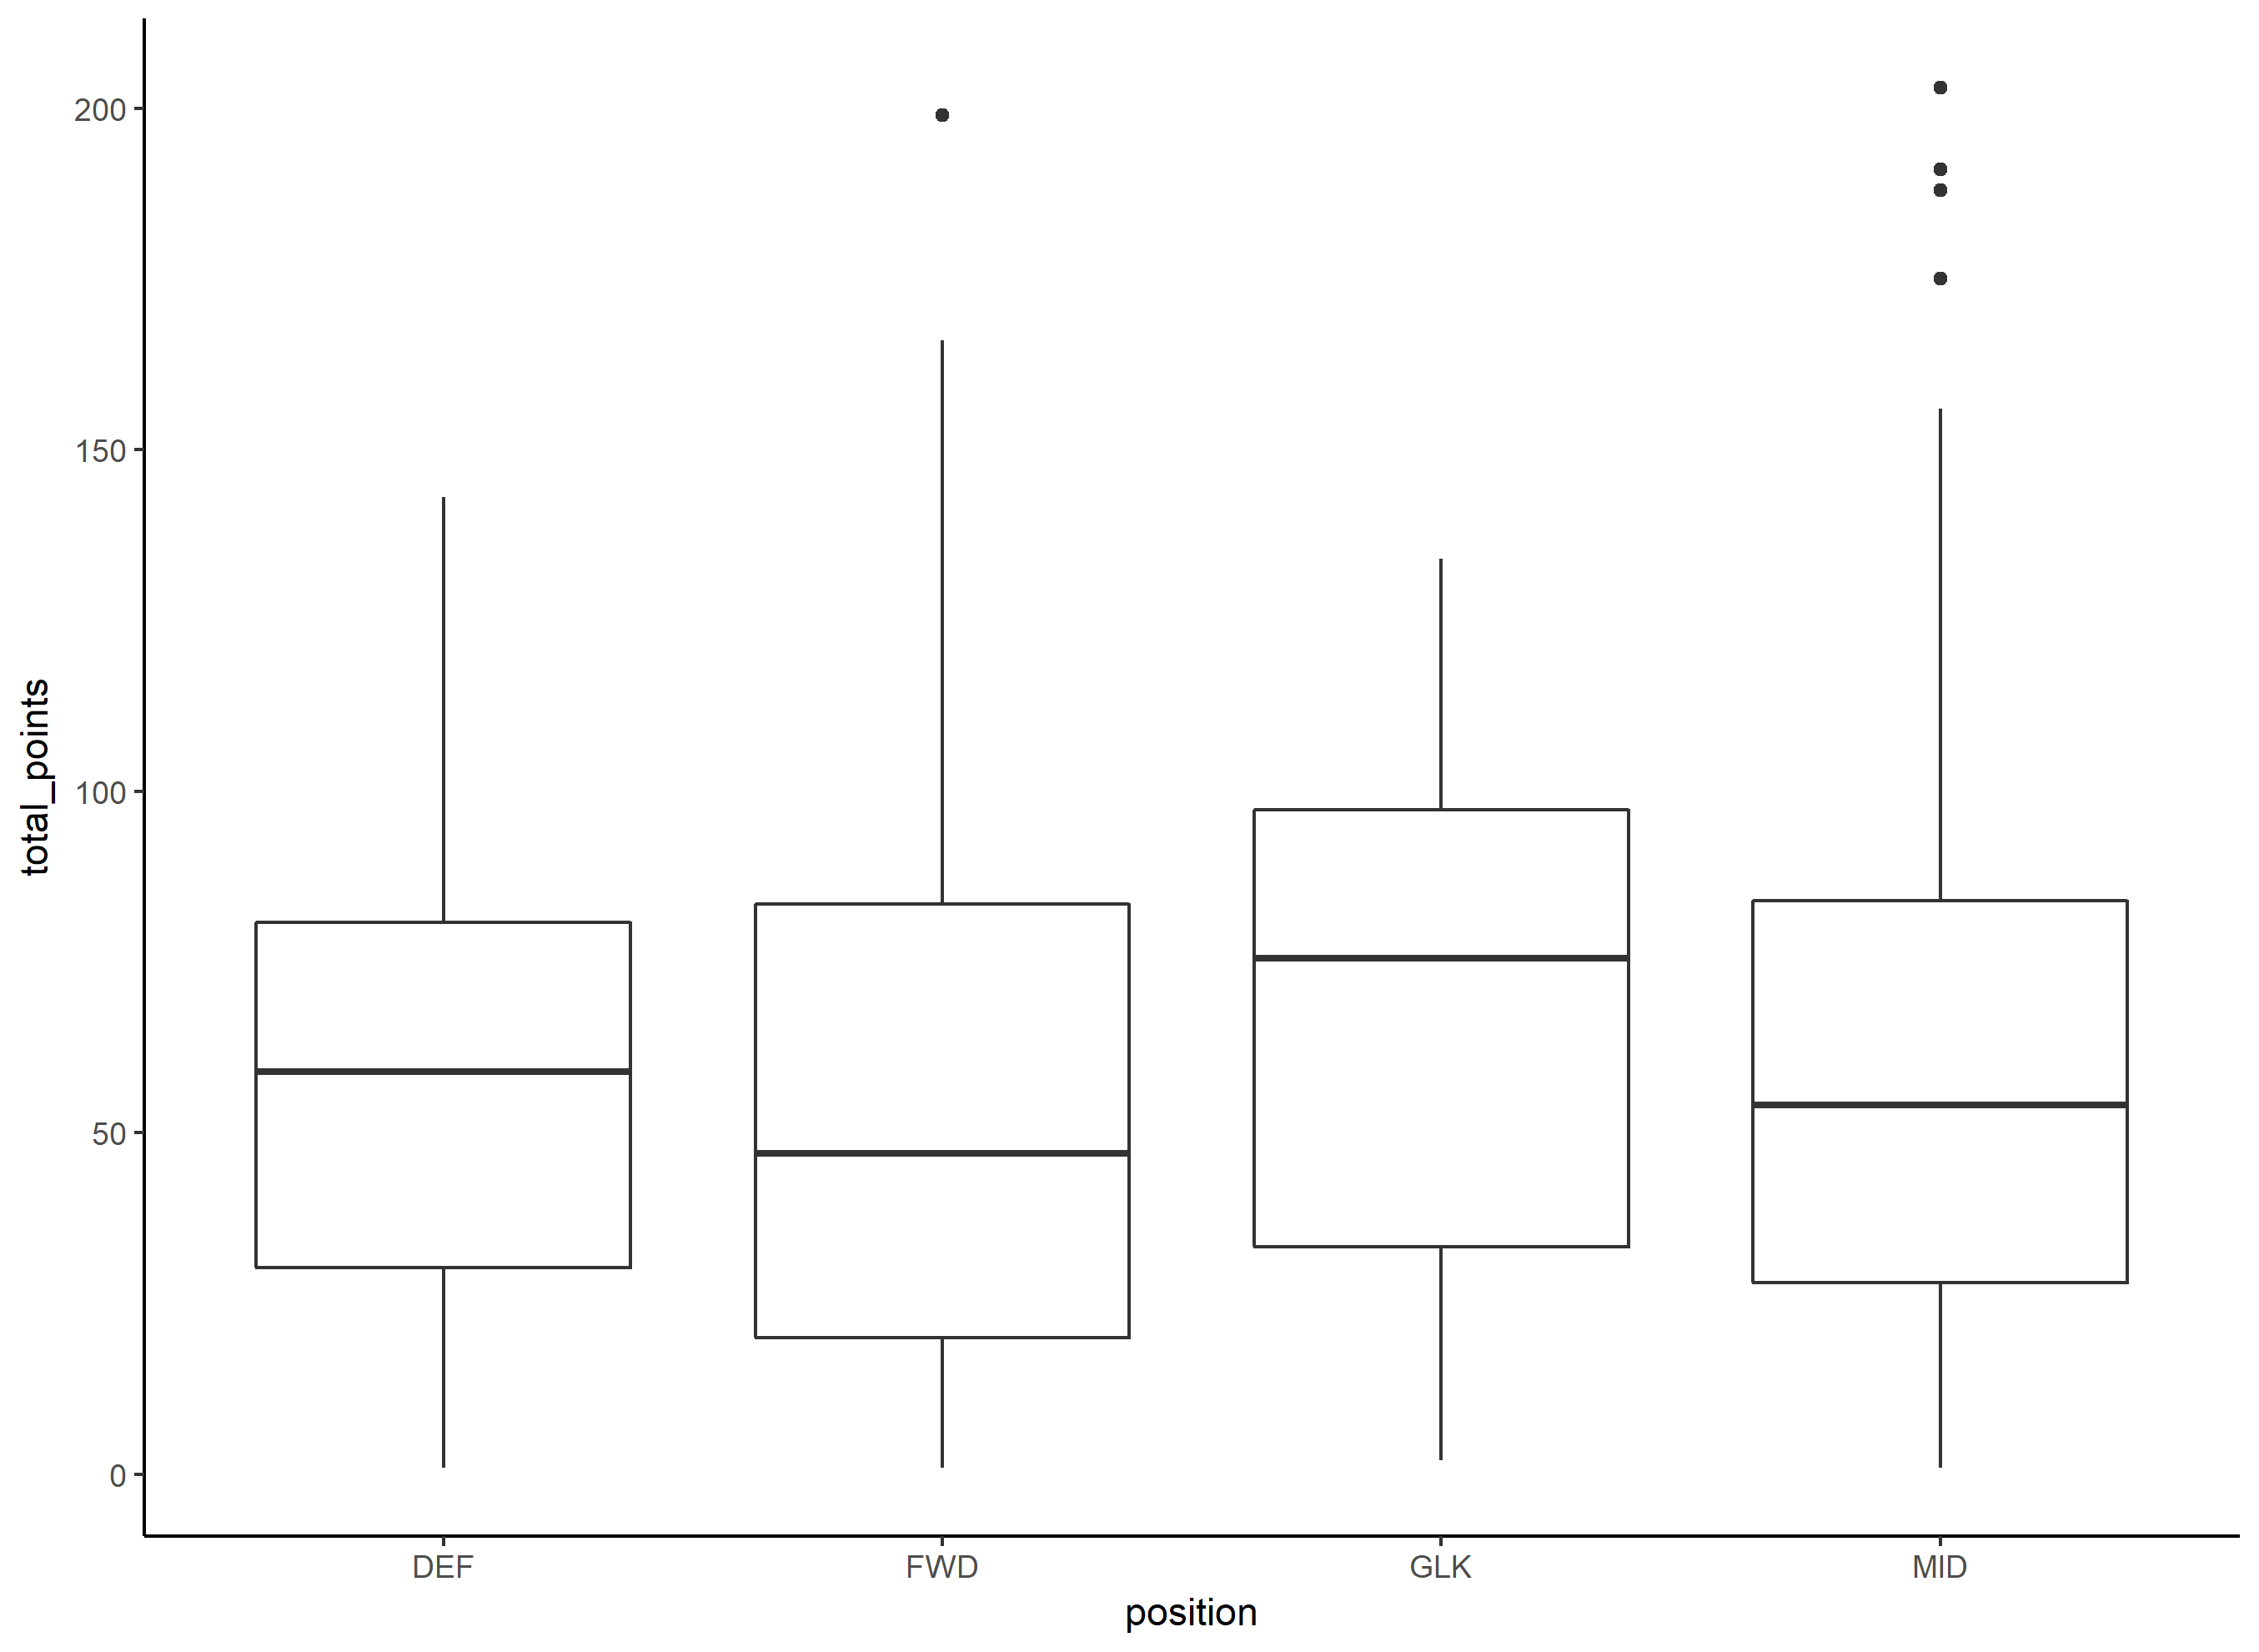
\includegraphics[scale=0.55]{fig/chapter_6/box_plot_positions.png}
    \caption{Box-plot of total points obtained in different positions over the 2016 season gameweek 1-32.}
\label{fig:box_plot}    
\end{figure}

\begin{figure}[H]
    \centering
    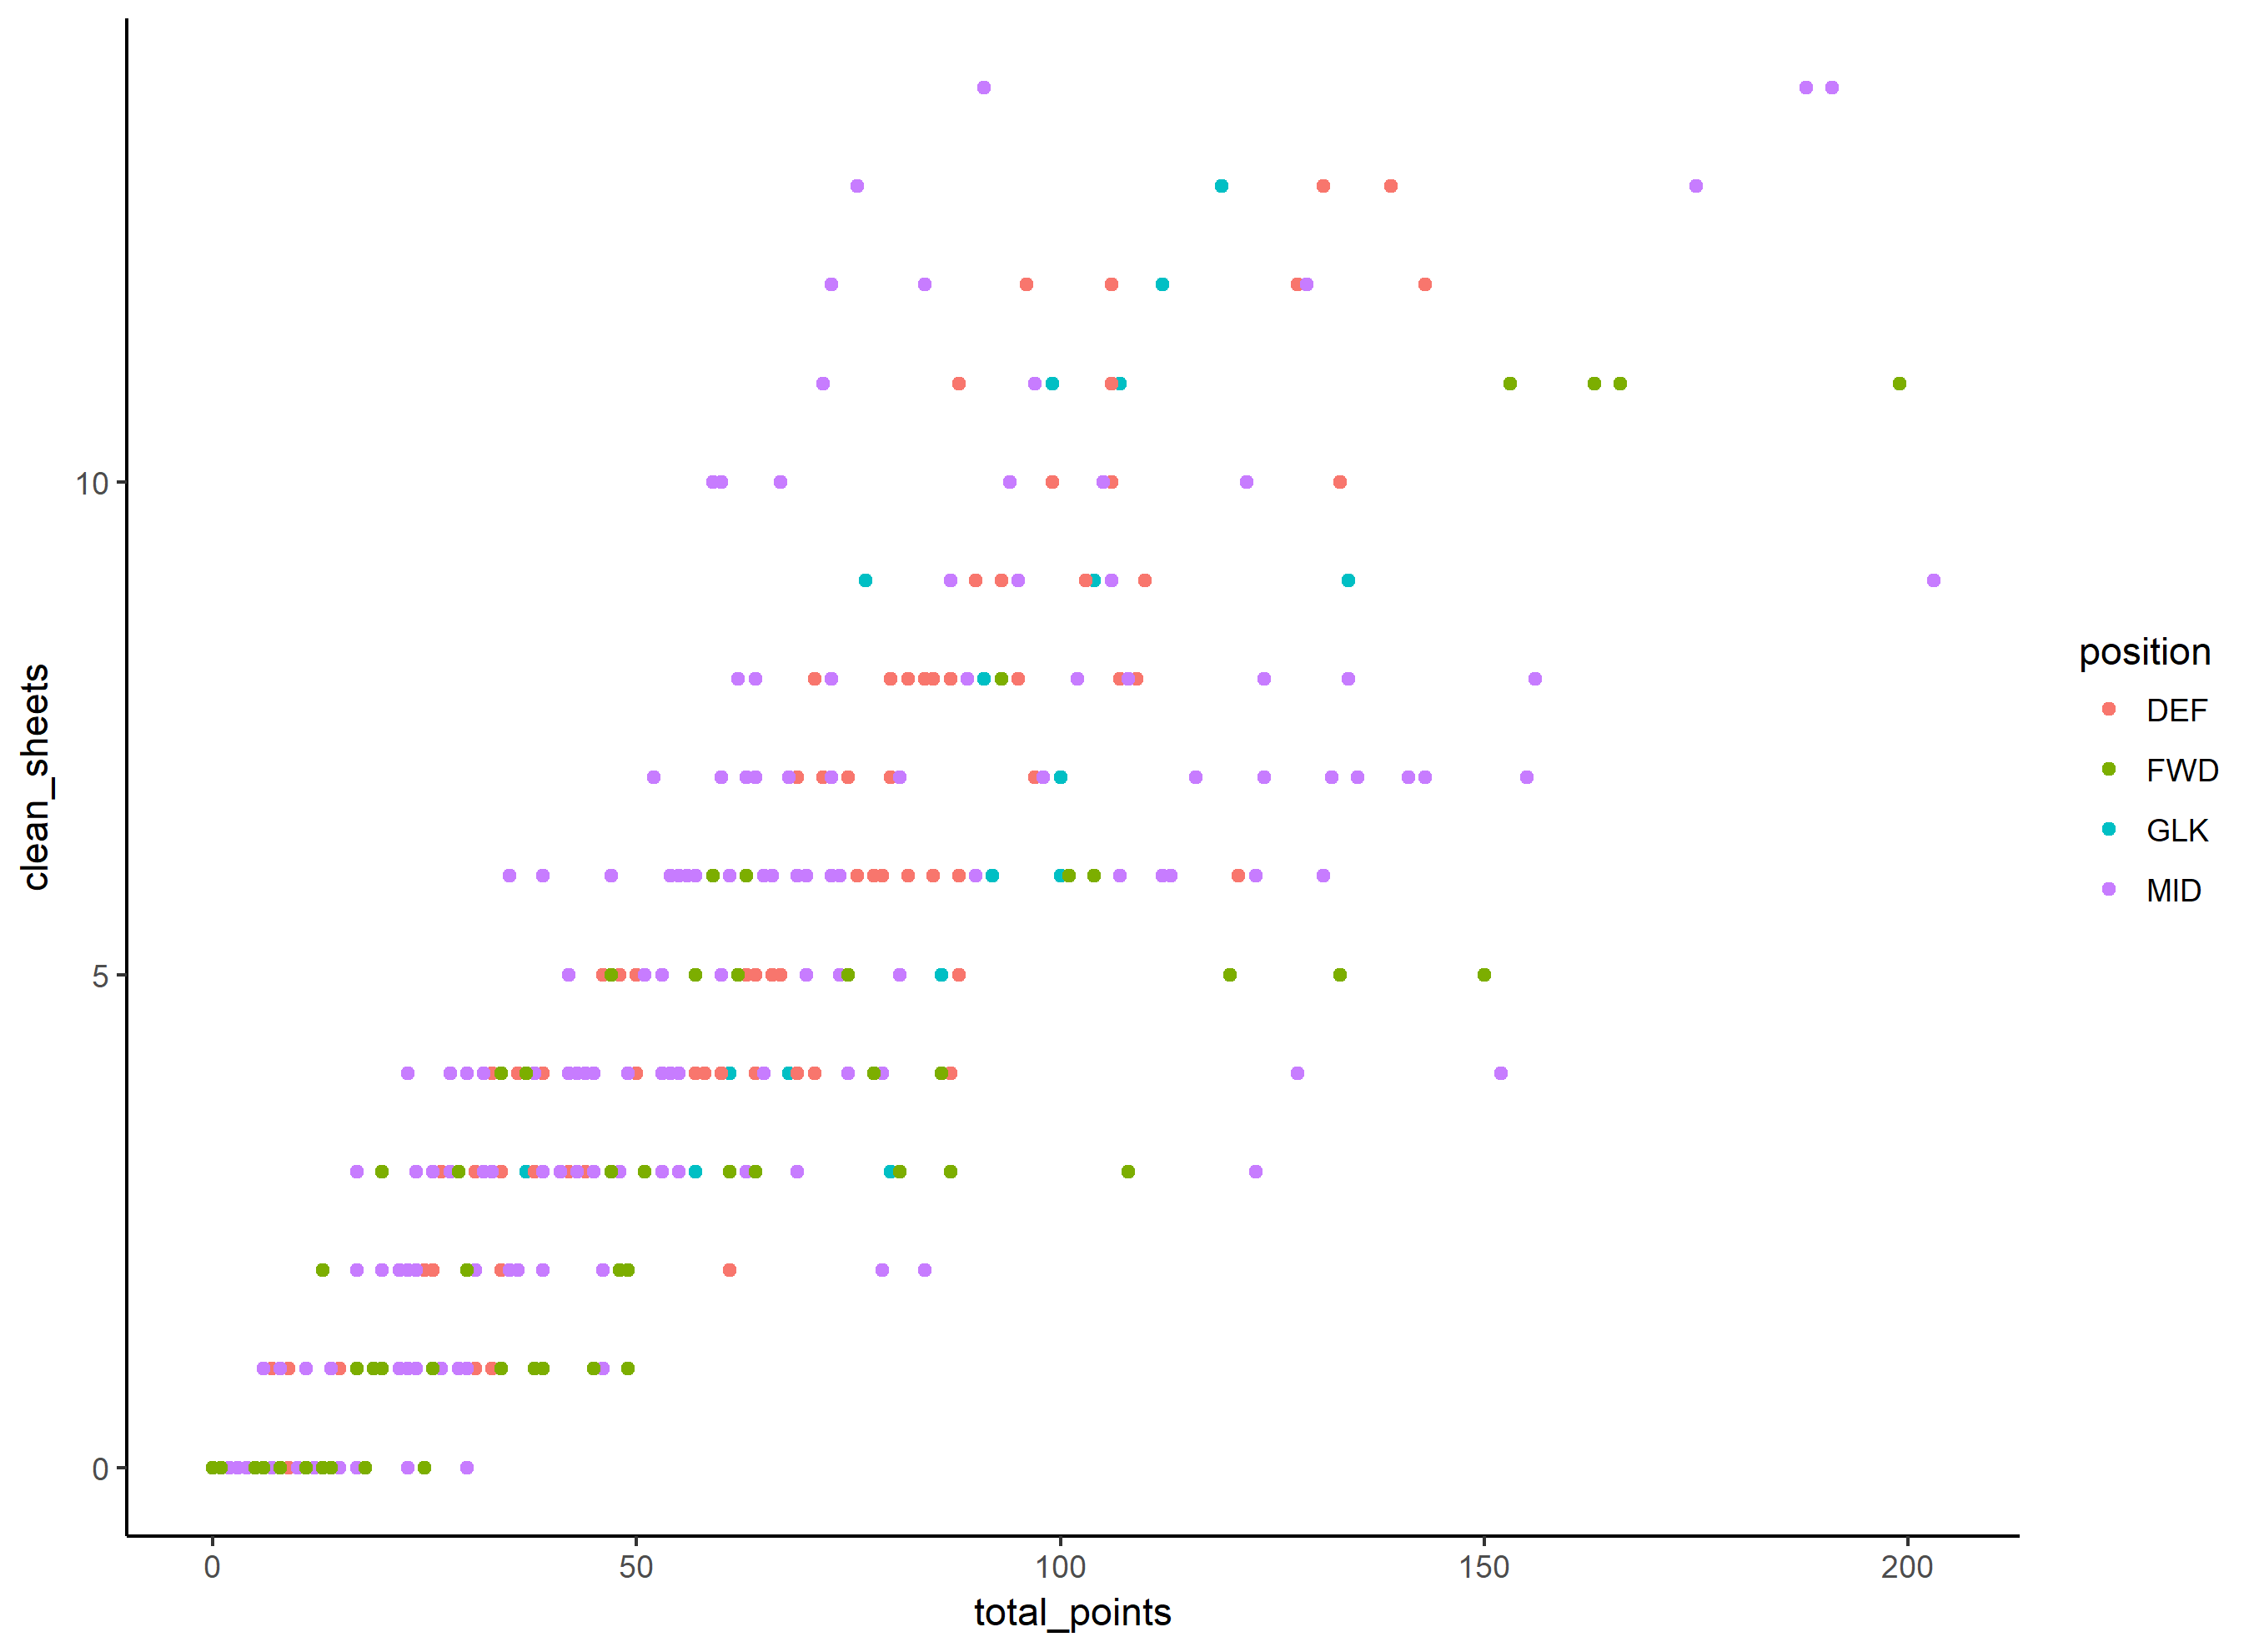
\includegraphics[scale=0.55]{fig/chapter_6/clean_sheet_tot_poins.png}
    \caption{Clean Sheets and Total points for different positions.}
\label{fig:cs_tot_p}    
\end{figure}

\begin{figure}[H]
    \centering
    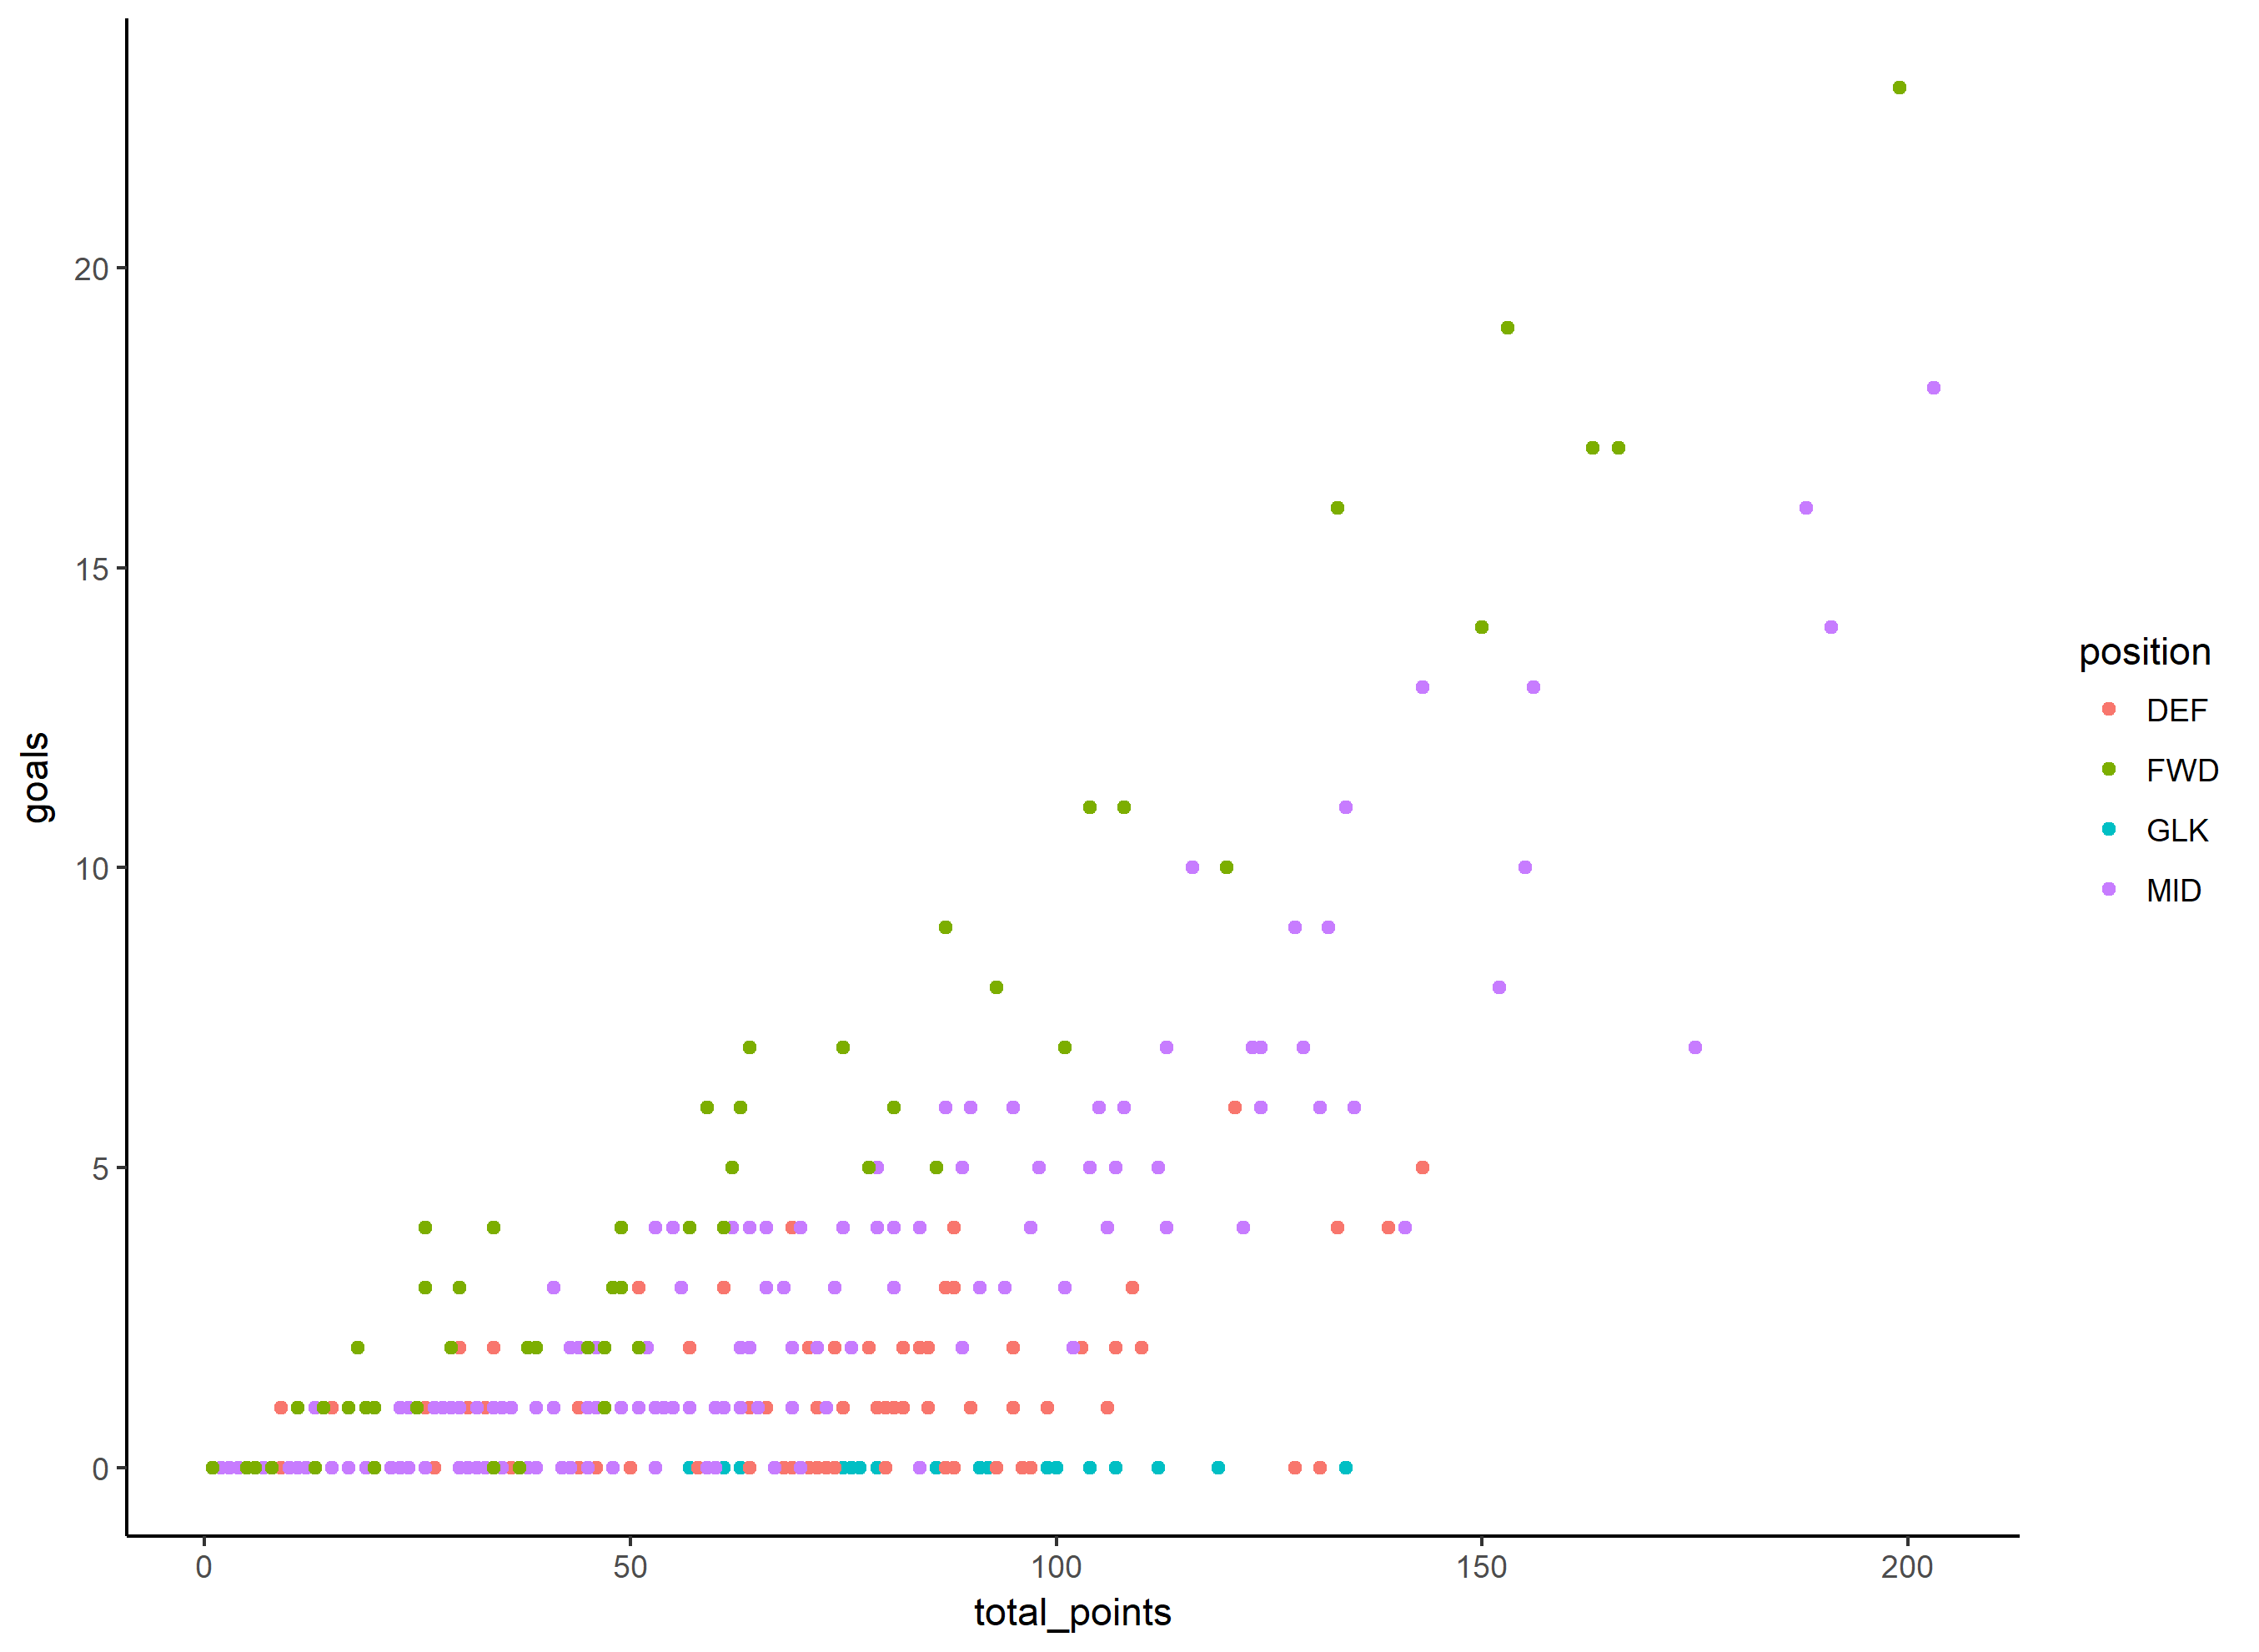
\includegraphics[scale=0.55]{fig/chapter_6/goals_tot_poins.png}
    \caption{Goals and Total points for different positions.}
\label{fig:goal_tot_p}    
\end{figure}

\subsubsection{Time Series of Points}

In order to determine if one should view the points a player obtains as a time series, the Durbin-Watson test and Ljung-Box test with lag 1-5 for autocorrelation are performed. In Table \ref{tab:auto_tests} the results of the tests are presented. Based on the results, 75\%-95\% of the players appear to have insignificant autocorrelation in their time-series of points at a significance level of 10 \%. This result should be interpreted carefully as the calculation is done for all players, and individual players may still display a time-dependency in points obtained. Regardless, we have decided to treat aggregates only, and neglect time-series effects in the regression. That is, the variable previous points is excluded from consideration. The methodology works as a complement to the Modified Average method, where only points in latest games are considered.

\begin{table}[H]
\centering
\begin{tabular}{lll}
Test            & \% significance level 10\% & \% significance level 5\% \\
Durbin-Watson   & 94 \% & 99 \%                                            \\
Ljung-Box lag 1 & 76 \% & 84 \%                                            \\
Ljung-Box lag 2 & 76 \% & 81 \%                                            \\
Ljung-Box lag 3 & 78 \% & 84 \%                                            \\
Ljung-Box lag 4 & 80 \% & 84 \%                                           \\
Ljung-Box lag 5 & 81 \% & 85 \%                                          
\end{tabular}
\caption{Summary of percentage of players with insignificant autocorrelation for different tests and significance levels.}
\label{tab:auto_tests}
\end{table}

\subsubsection{Variable Selection}

As described in Section \ref{Sol_approach_regression}, lasso regression is performed in order to conduct a variable selection. 80\% of the data of the 2016/2017 season is used for training, while the remaining 20 \% are used for testing. In the following, the variables deemed significant alongside a plot or RMSE against values of log($\lambda$) for each position is presented.

\newpar

\subsubsection{Goalkeepers}
As evident from Figure \ref{fig:goal_tot_p} no goalkeepers scored a goal in the up to gameweek 32 in the 2016/2017 English Premier League season. Furthermore, only one assist was provided. Therefore, we have decided not to consider these exploratory variables when performing the variable selection for goalkeepers. 


\begin{comment}

In Figures \ref{fig:lasso_GLK_1}, \ref{fig:lasso_DEF_1}, \ref{fig:lasso_MID_1} and \ref{fig:lasso_FWD_1} the RMSE of the test set is plotted against different values of log($\lambda$) for goalkeepers, defenders, midfielders and forwards respectively. Further, their significant variables are listed in Tables \ref{tab:sig_var_GLK_1}, \ref{tab:sig_var_DEF_1}, \ref{tab:sig_var_MID_1} and \ref{tab:sig_var_FWD_1} respectively.

\end{comment}

\begin{comment}


\begin{figure}[H]
    \centering
    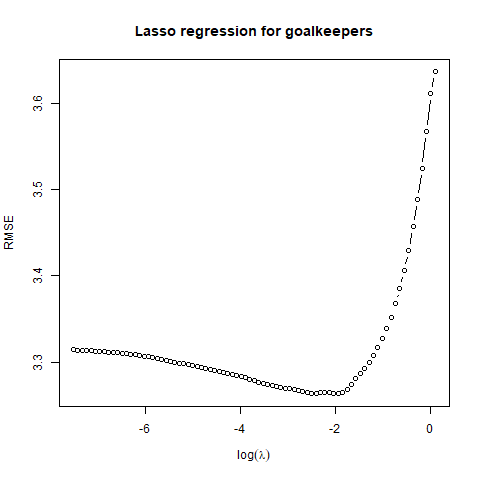
\includegraphics[scale=0.55]{fig/chapter_6/lasso_GLK.png}
    \caption{RMSE for different values of $\lambda$ for goalkeepers}
\label{fig:lasso_GLK}    
\end{figure}


\begin{table}[H]
\centering
\caption{Significant Variables for goalkeepers based on lasso regression and RMSE}
\label{tab:sig_var_GLK}
\begin{tabular}{l}
\textbf{Significant variables for goalkeepers }\\
Opponent                              \\
Team                                  \\
Cost                                  \\
Transfers in                          \\
Transfers out                         \\
Home/Away                             \\
Minutes played                        \\
Saves                                 \\
Clean Sheets                          \\
Assists                               \\
Own Goals                            
\end{tabular}
\end{table}

\end{comment}


\begin{table}[H]
\centering
\begin{minipage}{.5\textwidth}
  \centering
  \captionsetup{justification=centering}
    \begin{figure}[H]
        \centering
        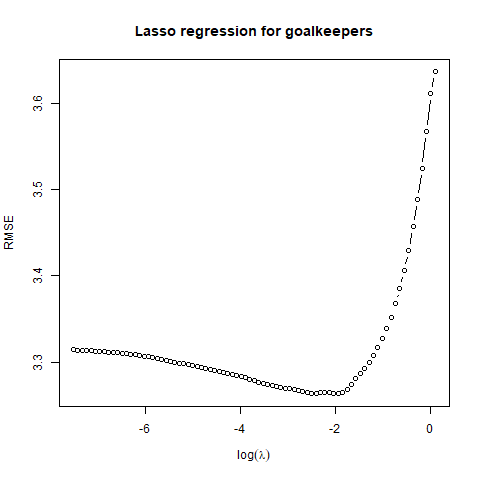
\includegraphics[scale=0.4]{fig/chapter_6/lasso_GLK.png}
    \end{figure}
    \captionof{figure}{RMSE for different values of $\lambda$ for goalkeepers}
    \label{fig:lasso_GLK_1}
\end{minipage}%
\begin{minipage}{.5\textwidth}
  \centering
  \captionsetup{justification=centering}
    \begin{tabular}{c}
    \\
    \textbf{Significant variables for Goalkeepers }\\
    \\
    \\
Opponent                              \\
Team                                  \\
Cost                                  \\
Transfers in                          \\
Transfers out                         \\
Home/Away                             \\
Minutes played                        \\
Saves                                 \\
Clean Sheets                          \\
Assists                               \\
Own Goals                            
    \\
    \\
    \\
    \\
\\


    \end{tabular}
\captionof{table}{Significant Variables for goalkeepers based on lasso regression and RMSE}
\label{tab:sig_var_GLK_1}
\end{minipage}
\end{table}

\begin{comment}
\textbf{Defenders}
In Figure \ref{fig:lasso_DEF} the RMSE of the test set is plotted against different values of $\lambda$. In Table \ref{tab:sig_var_DEF} the significant variables are listed
\end{comment}


\begin{table}[H]
\centering
\begin{minipage}{.5\textwidth}
  \centering
  \captionsetup{justification=centering}
    \begin{figure}[H]
        \centering
        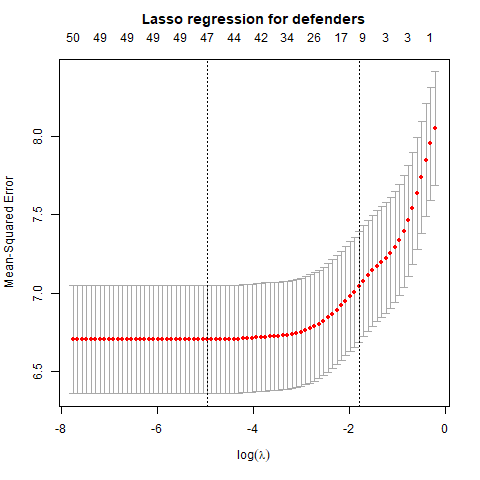
\includegraphics[scale=0.4]{fig/chapter_6/lasso_DEF.png}
    \end{figure}
    \captionof{figure}{RMSE for different values of $\lambda$ for defenders}
    \label{fig:lasso_DEF_1}
\end{minipage}%
\begin{minipage}{.5\textwidth}
  \centering
  \captionsetup{justification=centering}
    \begin{tabular}{c}
    \textbf{Significant variables for Defenders }\\
    \\
    \\
    \\
    
    Opponent                              \\
    Team                                  \\
    Cost                                  \\
    Transfers in                          \\
    Transfers out                         \\
    Home/Away                             \\
    Minutes played                        \\
    Yellow Cards                          \\
    Own Goals                             \\
    \\
    \\
    \\
    \\
   \\
   \\
    
    
    \end{tabular}
\captionof{table}{Significant Variables for midfielders based on lasso regression and RMSE}
\label{tab:sig_var_DEF_1}
\end{minipage}
\end{table}

\begin{comment}


\begin{figure}[H]
    \centering
    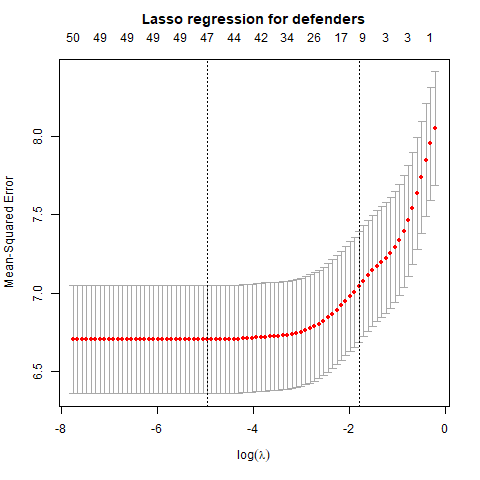
\includegraphics[scale=0.55]{fig/chapter_6/lasso_DEF.png}
    \caption{RMSE for different values of $\lambda$ for defenders}
\end{figure}

\begin{table}[H]
\centering
\caption{Significant Variables for defenders based on lasso regression and RMSE}
\begin{tabular}{l}
\textbf{Significant variables for Defenders }\\
Opponent                              \\
Team                                  \\
Cost                                  \\
Transfers in                          \\
Transfers out                         \\
Home/Away                             \\
Minutes played                        \\
Yellow Cards                          \\
Own Goals                                               
\end{tabular}
\end{table}

\end{comment}

\begin{comment}
\textbf{Midfielders}
In Figure \ref{fig:lasso_MID} the RMSE of the test set is plotted against different values of $\lambda$. In Table \ref{tab:sig_var_MID} the significant variables are listed
\end{comment}


\begin{table}[H]
\centering
\begin{minipage}{.5\textwidth}
  \centering
  \captionsetup{justification=centering}
    \begin{figure}[H]
        \centering
        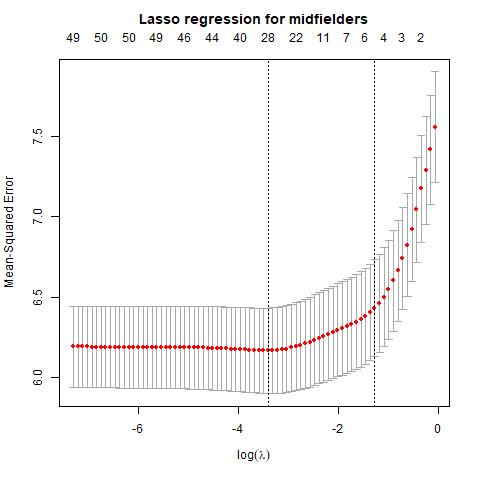
\includegraphics[scale=0.4]{fig/chapter_6/lasso_MID.png}
    \end{figure}
    \captionof{figure}{RMSE for different values of $\lambda$ for midfielders}
    \label{fig:lasso_MID_1}
\end{minipage}%
\begin{minipage}{.5\textwidth}
  \centering
  \captionsetup{justification=centering}
    \begin{tabular}{c}
    \\
    \textbf{Significant variables for Midfielders }\\
    \\
    \\
    \\
   Opponent                              \\
Team                                  \\
Cost                                  \\
Transfers in                          \\
Transfers out                         \\
Home/Away                             \\
Minutes played                        \\
Goals                                   \\
Penalty Misses                          \\
Clean Sheets                            \\
Assists                                 \\
\\
\\
\\

    \end{tabular}
\captionof{table}{Significant Variables for midfielders based on lasso regression and RMSE}
\label{tab:sig_var_MID_1}
\end{minipage}
\end{table}

\begin{comment}


\begin{figure}[H]
    \centering
    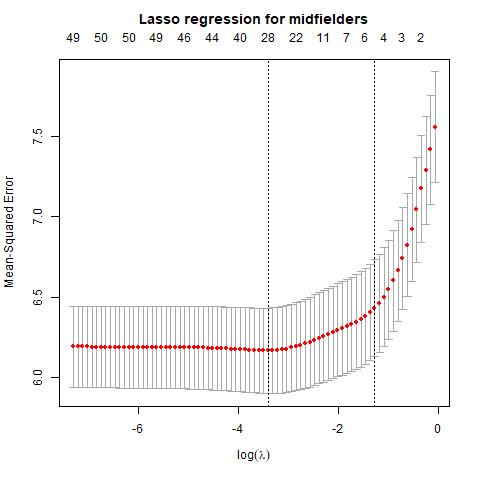
\includegraphics[scale=0.55]{fig/chapter_6/lasso_MID.png}
    \caption{RMSE for different values of $\lambda$ for midfielders}
\label{fig:lasso_MID}    
\end{figure}

\begin{table}[H]
\centering
\caption{Significant Variables for midfielders based on lasso regression and RMSE}
\label{tab:sig_var_MID}
\begin{tabular}{l}
\textbf{Significant variables for Midfielders }\\
Opponent                              \\
Team                                  \\
Cost                                  \\
Transfers in                          \\
Transfers out                         \\
Home/Away                             \\
Minutes played                        \\
Goals
        \\
Penalty Misses
        \\
Clean Sheets
        \\
Assists
\end{tabular}
\end{table}

\end{comment}

\begin{comment}
\textbf{Forwards}
In Figure \ref{fig:lasso_FWD} the RMSE of the test set is plotted against different values of $\lambda$. In Table \ref{tab:sig_var_FWD} the significant variables are listed
\end{comment}

\begin{table}[H]
\centering
\begin{minipage}{.5\textwidth}
  \centering
  \captionsetup{justification=centering}
    \begin{figure}[H]
        \centering
        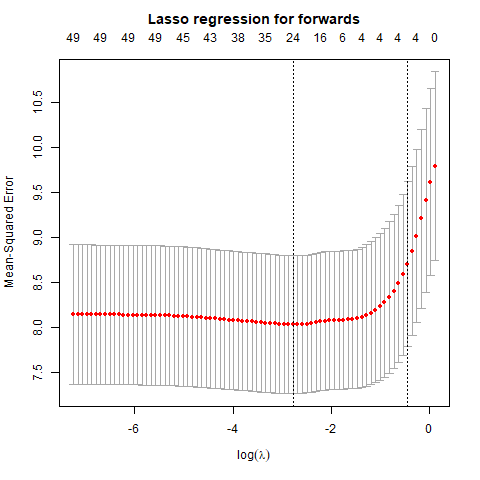
\includegraphics[scale=0.4]{fig/chapter_6/lasso_FWD.png}
    \end{figure}
    \captionof{figure}{RMSE for different values of $\lambda$ for forwards}
    \label{fig:lasso_FWD_1}
\end{minipage}%
\begin{minipage}{.5\textwidth}
  \centering
  \captionsetup{justification=centering}
    \begin{tabular}{c}
    \textbf{Significant variables for Forwards}\\
\\
\\    
\\
\\
Opponent                              \\
Team                                  \\
Cost                                  \\
Transfers in                          \\
Home/Away                             \\
Minutes played                        \\
Goals                                 \\
\\
\\
\\
\\
\\
\\
\\

 \end{tabular}
\captionof{table}{Significant Variables for forwards based on lasso regression and RMSE}
\label{tab:sig_var_FWD_1}
\end{minipage}
\end{table}

\begin{comment}

\begin{figure}[H]
    \centering
    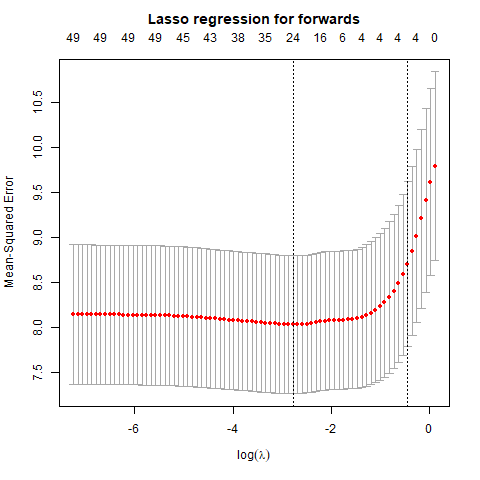
\includegraphics[scale=0.55]{fig/chapter_6/lasso_FWD.png}
    \caption{RMSE for different values of $\lambda$ for forwards}
\label{fig:lasso_FWD}    
\end{figure}

\begin{table}[H]
\centering
\caption{Significant Variables for forwards based on lasso regression and RMSE}
\label{tab:sig_var_FWD}
\begin{tabular}{l}
\textbf{Significant variables for Forwards}\\
Opponent                              \\
Team                                  \\
Cost                                  \\
Transfers in                          \\
Home/Away                             \\
Minutes played                        \\
Goals

\end{tabular}
\end{table}

\end{comment}

\textit{snakke litt mer om figurene og variablene}

\subsubsection{Model Selection}

For each position, a linear regression model is fitted based on the variables. A summary of each model is presented and a discussion of the signs of the constants is given. It is important to note that the model is continually "refitted" as new data becomes available. That is, the $\beta $s are updated. The variables remain the same. \newpar

\subsection{Odds}
In order to obtain necessary data, we have cooperated with Sportradar, a Norwegian company providing data for bookmakers. Sportradar delivers odds and probabilities of several sports events, including English Premier League. They have provided us with all the necessary probabilities, including result outcomes for each Premier League match as well as individual player probabilities. These data made all the computational work a lot easier, as Sportradar exported structured excel files containing all the necessary data. 
\newpar
Compared to the other two solution approaches, the player list is limited when calculating expected points using odds probabilities. The data from Sportradar was delivered post-season, which has affected the player list. Players that has been transferred or lend to other clubs during the 2017/2018 season are not considered. This is due to the fact that these players are no longer listed in Sportradar's database of Premier League players. In general, the reduced player list will not affect the results of the model, as the players that are lend out are typically lend to clubs in the English Championship division. Hence, these players were not consider good enough to contribute for the teams in the Premier League. However, some of the transfers might have an impact on the results. For instance, players like Philippe Coutinho and Michy Batshuayi are players that contributed with fantasy points in the first half of the season. Unfortunately, these players are not considered when using the odds approach, which is considered as a drawback of the approach.  
\newpar
As odds are primarily available for fixtures in the near future, in general for the upcoming gameweek, the suggested solution approach using odds is further limited. Hence, the sub-horizon in the optimization model is forced to be one gameweek. Compared to the other suggested methods, this is considered a great drawback.

\section{Gamechips} \label{exp_setup_gamechips}
Examining the fixtures list of this year's Premier League season, the game chips are played according to the solution approach suggested in section \ref{Ch.5_Game_chips}. As for the first Wildcard, our model is given the opportunity to play it in gameweek 9, where it can either choose to play it or to disregard it for the first half of the season. Hence, the model is not given the opportunity to play the first Wildcard in any other gameweeks than in gameweek 9. Further, the Triple Captain can only be played in gameweek 22, as this is the first double gameweek of the season. Moreover, we allow the Bench Boost to be played in the second double gameweek of the season, gameweek 34. Hence, the model is given the opportunity to play the second Wildcard in gameweek 33, preparing for the Bench Boost in the following gameweek. As we chose to play the Bench Boost in the double gameweek 34, we have chosen to allow the model to play a Free Hit in gameweek 31. This is a blank gameweek, were only 8 team are featured.


\section{Expected Value/Variance trade-off}
\label{exp_setup_Value_Variance}

\subsection{Variance in the proposed model}

In order to estimate the variance of each player and the correlation between players, their historical performances are considered. In order to obtain somewhat reliable estimations, data for the entire 2016/2017 season is used. Therefore, it is impossible to also find on optimal variance threshold using data on the 2016/2017 season. As a consequence, we have decided not to include expected value/variance trade-off in our proposed model. Instead, the effect of applying the constraint to out solution is described in Section ? and can provide a basis for future research and models.

\subsection{Variance Estimation}
The variance is calculated as the empirical variance in points obtained for each individual player. All previous available data from the 2016/2017 and the 2017/2018 season are used. That is, for gameweek 10 of the 2017/2018, data from all rounds of the 2016/2017 as well as the first nine round of the 2017/2018 season is used. This method of estimation is sensible for the Modified Average method. However, for the regression based model, the explanatory variables are assumed to explain some of the variance. Therefore it would be more suitable to estimate the variance based on the variance of the residuals. In the application described in Chapter 7, only the Modified Average method is considered. \newpar

\subsubsection{Special cases}
\textit{Lack of historical data}\newline
As previously discussed, complete historical data will not be available for all players for reasons such as promotion or transfers. If only one data-point is available for a player (i.e he has only played one match), it is impossible to calculate his variance. In these cases, the variance is set equal to the average variance of all other players. It is worth noting that this will only be an issue for one match, as more than one data-point will exist afterwards. The lack of data-points are obviously a limitation of the accuracy of the variance estimation, and constitutes a significant source of uncertainty. As the variance trade-off is considered a mean to reduce overall risk, another approach/improvement might consider only picking players with a history of say 10 matches. \newpar

\textit{Zero Variance}\newline
Some players have never played, but can be selected. These players might be interesting to choose for instance in order to fulfill the budget/number of players constraints. However, their empirical variance would equal 0. This is not desirable, as the future performance is not deterministic (they are \textit{not} analogous the the risk-free asset in a portfolio optimization setting). Therefore, their variance is set equal the lowest non-zero variance obtained by other players.

\subsection{Correlation Estimation}

In order to determine the correlation between two players on the same or opposing teams, historical data for the 2016/2017 season is considered. Note that data is aggregated such that only the correlation coefficient between different positions overall is considered. It is not calculated between individual players or teams. Therefore, the correlation between players in the same position in the same team is set equal to 1. The correlation between players that are not on the same team, nor facing each other in a game-week, is assumed to be 0.\newpar

Table \ref{tab:cor_team} and Table \ref{tab:cor_opp} show the correlation coefficient between different positions as well as the p-value from a Pearson's Product-Moment Correlation test where the alternative hypothesis is a correlation not equal to 0, for players of the same and opposing teams respectively. In the cases where the correlation is not significant (GLK FWD and DEF FWD of the same teams and GLK GLK of opposing teams), the correlation coefficient is set equal to 0. For the rest, the correlation coefficients ($\rho$) presented in the tables are used.

\begin{table}[H]
\centering
\caption{Correlation coefficient $\rho$ and p-value from significance test for the correlation between players of the same team}
\label{tab:cor_team}
\begin{tabular}{llll}
Position & Position & $\rho$    & p-value  \\
GLK      & DEF      & 0.689  & 2.20 E-16 \\
GLK      & MID      & 0.274  & 1.24 E-10 \\
GLK      & FWD      & 0.0288 & 0.519    \\
DEF      & MID      & 0.368  & 2.20 E-16 \\
DEF      & FWD      & 0.0578 & 0.176    \\
MID      & FWD      & 0.238  & 1.72 E-08
\end{tabular}
\end{table}

\begin{table}[H]
\centering
\caption{Correlation coefficient $\rho$ and p-value from significance test for the correlation between players of opposing teams}
\label{tab:cor_opp}
\begin{tabular}{llll}
Position & Position & $\rho$    & p-value  \\
GLK      & GLK      & 0.0162 & 0.759    \\
GLK      & DEF      & -0.106 & 0.0374   \\
GLK      & MID      & -0.312 & 2.78E-10 \\
GLK      & FWD      & -0.336 & 3.85E-16 \\
DEF      & DEF      & -0.319 & 2.35E-11 \\
DEF      & MID      & -0.447 & 2.20E-16 \\
DEF      & FWD      & -0.292 & 3.35E-09 \\
MID      & MID      & -0.254 & 1.00E-07 \\
MID      & FWD      & -0.136 & 0.00632 \\
FWD      & FWD      & -0.119 & 0.0218  
\end{tabular}
\end{table}